\documentclass[conference]{IEEEtran}
\usepackage{amsmath, amssymb, xcolor, graphicx, comment, algorithm, algpseudocode}
\usepackage{multirow}
\usepackage{tikz}
\usetikzlibrary{arrows.meta, positioning}
\usepackage{soul}
\DeclareMathOperator*{\argmax}{arg\,max}
\DeclareMathOperator*{\argmin}{arg\,min}
\DeclareMathOperator*{\sign}{\mbox{sign}}

\newcommand{\one}{\mathbf{1}}

\pagenumbering{arabic}

\usepackage{hyperref} 

\title{A Distributed Risk-Aware Bidding Strategy for Incorporating Renewable Generation into Real-Time Electricity Market}
\author{\IEEEauthorblockN{Tommy Truong, Zhihua Qu, and Marwan A. Simaan}
\IEEEauthorblockA{University of Central Florida}}

\begin{document}

\maketitle

\begin{abstract}
This paper proposes a risk-aware optimization framework in which firms' sensitivity to uncertainty serves as a tunable coordination variable. We show that, for a class of stochastic market games, there exists a structured relationship between firms' risk parameters and the resulting Nash equilibrium, such that appropriately chosen risk sensitivities induce Nash equilibria that lie on the Pareto frontier. Based on this insight, we develop a distributed algorithm that allows firms to estimate required aggregate quantities and adapt their risk parameters using only local communication and minimal information exchange. The proposed approach preserves the decentralized nature of the market: firms remain self-interested in their primary decisions, resulting in Pareto-optimal Nash equilibria, and convergence of the distributed algorithm follows from consensus theory under mild connectivity conditions.
\end{abstract}

%\begin{keywords}
{\it Keywords:} Risk-aware bidding, Nash equilibrium, Pareto efficiency, stochastic market, distributed optimization, renewable energy 
%\end{keywords}

\section{Introduction}

Competitive electricity markets operating under uncertainty exhibit a fundamental tension between individual rationality and collective efficiency.
Renewable energy operators in particular face this challenge acutely: their generation is stochastic and correlated through shared weather conditions,
their output forecasts are uncertain, and their bidding decisions must be submitted before real-time prices are known
\cite{dvorkin2020chance, wong2007pricing, mieth2020distribution}.
When each operator optimizes its own expected profit independently, the resulting Nash equilibrium generally fails to achieve socially optimal outcomes,
even when all firms behave rationally \cite{zhang2016competition, lee2015rational}.
This gap between Nash and Pareto-optimal performance is not merely a theoretical artifact---in markets with many correlated renewable operators,
it translates directly into foregone collective profit and inefficient price signals \cite{asplund2002risk, wambach1999bertrand}.

Existing studies on stochastic Cournot and oligopoly games have examined the impact of uncertainty and risk preferences on equilibrium outcomes,
but typically treat risk attitudes as fixed exogenous parameters \cite{cheng2002bertrand, sakai1989risk, gulpinar2014analysis}.
Under this assumption, the equilibrium is determined once risk preferences are assigned, leaving no room to steer outcomes.
Separately, Pareto efficiency has been studied through centralized optimization or cooperative formulations that require full information sharing
\cite{hobbs2001individual, zhao2010social, su2018integrated}.
These approaches are impractical in deregulated markets where operators are self-interested and unwilling to disclose private cost and forecast data.
The key question that remains unaddressed is whether Nash equilibrium behavior can be reconciled with Pareto-optimal outcomes
\emph{without} centralized coordination or private information disclosure.

This paper answers that question affirmatively by identifying risk sensitivity itself as the coordination variable.
We show that, for a class of stochastic renewable energy market games, there exists a structured relationship between the operators'
risk parameters and the resulting Nash equilibrium bidding strategies, such that appropriately chosen risk levels induce Nash equilibria
that lie on the Pareto frontier.
In this sense, risk is not merely a preference parameter but a mechanism through which self-interested agents can be guided
toward efficient collective outcomes without violating incentive compatibility.
This perspective connects to the mechanism design literature~\cite{hurwicz1960optimality,myerson1979incentive}: rather than redesigning the market structure, the utility prescribes risk parameters that act as a voluntary coordination instrument, inducing Pareto-efficient Nash behavior without coercive transfers or centralized side payments.

The key enabler for a distributed implementation is that the Pareto condition depends only on the \emph{aggregate} risk level
across operators, not on individual bidding strategies directly.
This means coordination reduces to reaching consensus on a single scalar quantity,
which can be accomplished through local communication without revealing private information.
Building on this insight, we develop a distributed consensus-based algorithm that allows each operator to estimate the required
aggregate quantities and set its risk parameter using only neighborhood communication \cite{molzahn2017survey, yang2019survey}.
Analytical results establish existence and explicit characterization of Pareto-optimal Nash equilibria,
and convergence of the distributed algorithm is established under a mild connectivity condition.
A numerical example illustrates how risk-aware adaptation shifts equilibrium behavior from inefficient Nash outcomes to Pareto-optimal payoffs,
and a sensitivity analysis quantifies the performance impact of physical bid constraints.

The remainder of the paper is organized as follows.
Section~II formulates the stochastic market model and risk-aware objectives.
Section~III characterizes the Nash equilibrium under fixed risk parameters.
Section~IV establishes conditions under which Nash equilibria achieve Pareto efficiency through structured risk allocation.
Section~V presents a distributed algorithm based on consensus to realize these outcomes.
Numerical results are provided in Section~VI, followed by concluding remarks in Section~VII.

\section{Problem Formulation}

In this paper, we consider the simple case that all traditional generation assets are owned by a single utility company\footnote{The proposed results apply to the general case of multiple utility companies of individual cost functions except for notational complexity.} while renewable generation is operated by individual entities (one of which could be the utility company). And, the utility company and the renewable generation operators are the participants in both day-ahead and real-time electricity markets for profit. 

\begin{figure}[hbt!]
\centering
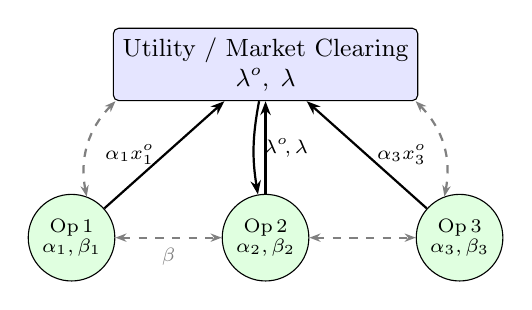
\begin{tikzpicture}[
  scale=0.88,
  mkt/.style={draw, rectangle, rounded corners=2pt, fill=blue!10,
              minimum width=3.4cm, minimum height=0.7cm,
              font=\small, align=center},
  op/.style={draw, circle, fill=green!12, minimum size=1.1cm,
             font=\scriptsize, align=center, inner sep=1pt},
  arr/.style={-{Stealth[length=5pt]}, thick},
  comm/.style={{Stealth[length=4pt]}-{Stealth[length=4pt]}, dashed, gray, thick}
]
\node[mkt] (util) at (0, 3.1) {Utility / Market Clearing\\$\lambda^o,\;\lambda$};
\node[op] (op1) at (-2.8, 0.6) {Op\,1\\[-1pt]$\alpha_1,\beta_1$};
\node[op] (op2) at (0,   0.6) {Op\,2\\[-1pt]$\alpha_2,\beta_2$};
\node[op] (op3) at ( 2.8, 0.6) {Op\,3\\[-1pt]$\alpha_3,\beta_3$};
% Bid submission
\draw[arr] (op1) -- node[left,  font=\scriptsize]{$\alpha_1 x_1^o$} (util);
\draw[arr] (op2) --                                                   (util);
\draw[arr] (op3) -- node[right, font=\scriptsize]{$\alpha_3 x_3^o$} (util);
% Price return
\draw[arr, bend right=10] (util) to
      node[right, font=\scriptsize]{$\lambda^o\!,\lambda$} (op2);
% Consensus communication graph
\draw[comm] (op1) -- node[below, font=\scriptsize]{$\beta$} (op2);
\draw[comm] (op2) -- (op3);
\draw[comm, bend left=28]  (op1) to (util);
\draw[comm, bend right=28] (op3) to (util);
\end{tikzpicture}
\caption{System and communication structure. Solid: bid submission and price return. Dashed: consensus links for Algorithm~\ref{alg:dist_risk_aware}.}
\label{fig:system_schematic}
\end{figure}

In an electricity market, utility aims to optimize a composite objective function in the form of 
\begin{equation} 
J(P_g) = a_2 P_g^2 + a_1 P_g + a_0, \label{eq:Jm}
\end{equation}
where $a_i$ are cost coefficients, and $P_g$ is the aggregated power of traditional generation. For simplicity, marginal costs of operating renewables and battery storage sites are modeled as zero, and hence they need not to be included explicitly in objective function \eqref{eq:Jm}. 

Let $n$ denote the total number of renewable generation operators and $\Omega=\{1,\cdots,n\}$ be the index set. For the day-ahead market, their renewable generations, $P_j$ for $j\in\Omega$, are modeled as stochastic variables, and similarly the grid total load $P_L$ is also modeled as a stochastic variable. Let us form the whole vector of random variables as 
\begin{equation} 
x = \begin{bmatrix} P_1 & \cdots & P_n & P_L \end{bmatrix}^T.  \label{eq:x}
\end{equation}
We assume that probability distribution of random vector $x$ is Gaussian as follows:
\[ f(x) = (2\pi)^{-\frac{n+1}{2}}\Sigma^{-\frac{1}{2}} e^{-\frac{1}{2}(x-x^o)^T\Sigma^{-1}(x-x^o)},  \]
where  $x^o=\mathbb{E}[x]$ is the vector of forecast (for the day-ahead market), and 
\begin{eqnarray*}
\Sigma & = & \mathbb{E}[(x-x^o)(x-x^o)^T] \\
& = & \begin{bmatrix} \sigma_{11} & \cdots & \sigma_{1n} & \sigma_{1L} \\ \vdots & \cdots & \vdots & \vdots \\ \sigma_{n1} & \cdots & \sigma_{nn} & \sigma_{nL} \\ \sigma_{1L} & \cdots & \sigma_{nL} & \sigma_{LL}
\end{bmatrix},  
\end{eqnarray*}
is the covariance matrix with $\sigma_{ij}=\sigma_{ji}$. In the covariance matrix, the last row and column correspond to covariances between the renewable generations and the load while $\sigma_{LL}=\sigma_L^2>0$ is the variance of the load. It is known that
$\sigma_{ii}=\sigma_i^2>0$, $\sigma_{ij}=\rho_{ij}\sigma_i\sigma_j$, $\sigma_{iL}=\rho_{iL}\sigma_i\sigma_L$, where $\rho_{ij},\rho_{iL}\in[0,1]$. Typically, $\rho_{ij},\rho_{iL}\not=0$ because renewable generations and load are correlated through the projected weather condition.

The Gaussian model is adopted for notational consistency with standard stochastic Cournot frameworks, but the key results of this paper require only that $x$ have finite mean $x^o$ and covariance $\Sigma$. The risk penalty $\mathbb{E}[(\lambda-\lambda^o)^2]$ and total profit $\Pi$ both expand as polynomials in the bidding coefficients with moment-based coefficients determined entirely by $x^o$ and $\Sigma$ (see~\eqref{eq:Pi_j_exp} and~\eqref{eq:sigma_lambda}), so Theorems~1--2 and Corollaries~1--5b hold for any joint distribution with finite second moments, including Weibull wind and beta solar distributions common in practice. Gaussianity would be needed only for distributional risk measures beyond variance (e.g., CVaR) or for characterizing higher moments of individual profits, which are deferred to future work.

The day ahead market clears the projected aggregated power generation $P_g^o$ and its associated price $\lambda^o$ by minimizing $J(P_g^o)$ under the following power balance constraint:
\begin{equation} 
P_g^o + \sum_{j\in\Omega} \alpha_j x_j^o  = x_{n+1}^o, \label{eq:DA_power}
\end{equation}
where $x_{n+1}^o=P_L^o$, $\alpha_j\in[0,1]$ if no overbidding is allowed or $\alpha_j\in[0,\infty)$ if overbidding is permitted, and $\alpha_j x_j^o =\alpha_j P_j^o$ represent the bids by the renewable generation operators into the day-ahead market. Similarly, the real-time market clears the aggregated power generation $P_g$ and its associated price $\lambda$ by minimizing $J(P_g)$ under the following real-time power balance constraint:
\begin{equation} 
P_g + \sum_{j\in\Omega} x_j   = x_{n+1}. \label{eq:RT_power}
\end{equation}
It is well known that, with global information, day-ahead price $\lambda^o$ and real-time $\lambda$ are the dual variables associated with constraints \eqref{eq:DA_power} and \eqref{eq:RT_power}, respectively. 

The renewable generation operators aim to maximize the following objectives\footnote{Strictly speaking, we should use $J_i^{\prime} = \Pi_i - \beta_i \mathbb{E}[(\Pi_i - \mathbb{E}[\Pi_i])^2]$ which also yields a second-order polynomial in $\alpha_i$ as does \eqref{eq:J_i} but involves calculations of higher moments. Accordingly, \eqref{eq:J_i} is adopted instead.} individually:
\begin{subequations}
\begin{equation} 
J_i = \Pi_i - \beta_i \mathbb{E}[(\lambda - \lambda^o)^2], \label{eq:J_i}
\end{equation}
where $\beta_i\in\mathbb{R}$, 
\begin{equation} 
\Pi_i %= \lambda^o \alpha_i P_i^o + \mathbb{E}[\lambda (P_i - \alpha_i P_i^o)] 
= \lambda^o \alpha_i x_i^o + \mathbb{E}[\lambda (x_i - \alpha_i x_i^o)], \label{eq:Pi_i}
\end{equation}
\end{subequations}
and the pair $\{\alpha_i, \; \beta_i\}$ represents the bidding strategy of the $i$-th operator into the electricity markets. Throughout this paper, $J_i$ exclusively denotes the risk-aware objective defined in~\eqref{eq:J_i}; the special case $\beta_i=0$ reduces $J_i$ to pure expected profit maximization and is referred to as the risk-neutral strategy. If $\beta_i=0$ is chosen, the $i$-th entity aims to maximize its average profit from the total revenues from participating in the day ahead and real time markets. By selecting $\beta_i>0$, the $i$-th entity also attempts to reduce its profit variation by suppressing variations of real time price $\lambda$ around day ahead price $\lambda^o$.  By choosing $\beta_i<0$, the $i$th entity tries to maximize its profit by encouraging more variations of real time price $\lambda$ around day ahead price $\lambda^o$. In other words, the $i$-th entity is risk averse if $\beta_i>0$ and risk seeking if $\beta_i<0$.

The risk-aware bidding strategy $\{\alpha_i,\beta_i\}$ offers four advantages: (i) achieving Pareto-optimal Nash equilibria that maximize the total profit $\sum_{i\in\Omega} \Pi_i$; 
% (equivalently, maximizing $g(\alpha_1^*,\ldots,\alpha_n^*)$ as defined in \eqref{eq:G});
(ii) enabling distributed implementation without centralized coordination; (iii) maintaining incentive compatibility as firms remain self-interested; and (iv) preserving privacy through minimal information exchange. Power grid congestion is not considered in the paper but can be considered.

\section{Centralized Risk-Aware Solution Under Global Information}

The electricity markets are bi-level optimization problems linked together by dual variables. At the upper level, they are quadratic optimization problems with equality constraints, that is, the markets perform their economic dispatch with the following Lagrangians: 
\begin{subequations}
\begin{equation} 
L^o = a_2(P_g^o)^2+a_1P_g^o+a_0 + \lambda^o\left(x_{n+1}^o- P_g^o-\sum_{j\in\Omega} \alpha_j x_j^o \right), \label{eq:L*}
\end{equation}
\begin{equation} 
L = a_2P_g^2+a_1P_g+a_0 + \lambda\left(x_{n+1}-P_g-\sum_{j\in\Omega} x_j\right). \label{eq:L}
\end{equation}
\end{subequations}
Applying the first-order optimality condition to the Lagrangians yields the following solutions for the prices:
\begin{subequations}
\begin{equation} 
\lambda^o = 2a_2P_g^o +a_1 = 2a_2\left(x_{n+1}^o-\sum_{j\in\Omega} \alpha_j x_j^o \right) +a_1 , \label{eq:lambda*}
\end{equation}
\begin{equation} 
\lambda = 2a_2P_g+a_1=2a_2\left(x_{n+1}-\sum_{j\in\Omega} x_j \right) + a_1. \label{eq:lambda}
\end{equation}
\end{subequations}

The lower level optimization problems are also quadratic, and the centralized solutions under global information are summarized into the following lemma and theorem. Lemma 1 provides the solution of cooperative optimization when all the entities bind themselves together and act as one. In this case, the best outcome for the group is achieved under the risk neutral strategy.

\noindent \textbf{Lemma 1:} {\it Consider the case that all renewable generation entities form a coalition by sharing all the information and setting $\alpha_i=\alpha$ and $\beta_i=\frac{1}{n}\beta$, respectively. Then, for any choice of $\beta\in[-(4a_2)^{-1},\; +\infty)$, the optimal bidding strategy to optimize objective function $\sum_i J_i$ with $J_i$ in \eqref{eq:J_i} is
\begin{equation}
\alpha^* = \frac{1 + 4a_2 \beta}{2(1 + 2a_2\beta)}.
\label{eq:alpha_1}
\end{equation}
In addition, by further choosing $\beta_i$ to optimize $\sum_i \Pi_i$ with $\Pi_i$ in \eqref{eq:Pi_i}, the optimal bidding strategy $\{\alpha^*, \; \beta^*\}$ is given by}
\begin{equation}
\alpha^*  =  \frac{1}{2}, \quad
\beta^*  =  0.
\label{eq:optimal_1}
\end{equation}

\noindent \textbf{Proof:} It follows from \eqref{eq:Pi_i} and \eqref{eq:lambda*} that, if $\alpha_i=\alpha$, 
\begin{eqnarray*}
\Pi_r & = & \sum_{j\in\Omega} \Pi_j = \lambda^o \alpha x_r^o +  \mathbb{E}[\lambda (x_r-\alpha x_r^o)] \\
 \lambda^o   & = & 2a_2\left(x_{n+1}^o-\alpha x_r^o \right) +a_1,
\end{eqnarray*}
where $x_r = \sum_{j\in\Omega} x_j$ is the total renewable generation, and $x_r^o = \sum_{j\in\Omega} x_j^o$. Substituting \eqref{eq:lambda} into the above equations yields
\begin{eqnarray}
\Pi_r & = &  [2a_2\left(x_{n+1}^o-\alpha x_r^o \right) +a_1] \alpha x_r^o \nonumber \\
&& + \mathbb{E}[(2a_2\left(x_{n+1}-x_r \right) + a_1)(x_r-\alpha x_r^o)] \nonumber \\
  & = & 2a_2\alpha(1-\alpha)(x_r^o)^2 +a_1x_r^o  + 2a_2\mathbb{E}[\left(x_{n+1}x_r-x_r^2 \right)] \nonumber\\
   & = & 2a_2\alpha(1-\alpha)(x_r^o)^2 +a_1x_r^o \nonumber \\
   && + 2a_2\left(x_{n+1}^ox_r^o+\sigma_{rL}-(x_r^o)^2-\sigma_r^2 \right), \label{eq:Pi_r_exp}
\end{eqnarray}
where $\sigma_{rL}\triangleq\sum_{i\in\Omega}\sigma_{iL}$ is the total renewable-load cross-covariance, $\one$ is the $n$-dimensional column vector of $1$s, and
\begin{eqnarray*}
    \sigma_r^2 & = & \mathbb{E}[(x_1+\cdots+x_n-(x_1^o+\cdots+x_n^o))^2] \\
    & = & \mathbb{E}[ \one^T (x_r-x_r^o)(x_r-x_r^o)^T\one] \\
    & = & \one^T \Sigma_r \one \;=\; \sum_{i\in\Omega}\sum_{j\in\Omega} \sigma_{ij},
\end{eqnarray*}
where $x_r = [x_1,\ldots,x_n]^T$ is the $n$-vector of renewable generations and $\Sigma_r$ is the upper-left $n\times n$ subblock of $\Sigma$ containing only the renewable-to-renewable covariances $\sigma_{ij}$, $i,j\in\{1,\ldots,n\}$.
On the other hand, it follows from \eqref{eq:J_i}, \eqref{eq:lambda*}, and \eqref{eq:lambda} that, if $\beta_i = \frac{1}{n}\beta$,
\begin{eqnarray*}
J_r & = & \sum_{j\in\Omega} J_j \\
 & = & \Pi_r  - \beta \mathbb{E}[2a_2 (x_{n+1}-x_{n+1}^o -x_r +\alpha x_r^o)^2] \\
 & = & 2a_2\alpha(1-\alpha)(x_r^o)^2  - 4a_2^2  \beta  (1-\alpha)^2 (x_r^o)^2 \\
 & & +a_1x_r^o + 2a_2\left(x_{n+1}^ox_r^o+\sigma_{rL}-(x_r^o)^2-\sigma_r^2 \right)\\
 && - 4a_2^2  \beta (\sigma_L^2+\sigma_r^2 - 2\sigma_{rL}). 
\end{eqnarray*}
Using the above expression, taking the partial derivative of $J_r$ with respect to $\alpha$, and setting the partial derivative to zero yield optimal bidding strategy \eqref{eq:alpha_1}. 

Substituting solution \eqref{eq:alpha_1} into 
\eqref{eq:Pi_r_exp} and differentiating $\Pi_r$ with respect to $\beta$ yields
\[ \frac{\partial \Pi_r}{\partial \beta} = - 2a_2(x_r^o)^2\frac{4a_2^2\beta}{(1+2a_2\beta)^3}, \]
which yields the optimal bidding strategy \eqref{eq:optimal_1}. This completes the proof. \hfill $\Box$

It follows from \eqref{eq:alpha_1} that
\[ \lim_{\beta\rightarrow-1/(4a_2)} \alpha = 0, \quad  \lim_{\beta\rightarrow0} \alpha = 0.5, \quad \lim_{\beta\rightarrow +\infty} \alpha = 1. \]
Since $\alpha\in[0,1]$, the design parameter $\beta$ translates an operator's risk tolerance level into a specific choice of $\alpha$ value. Although the specific value corresponding to the risk-neutral choice may differ, this translation is applicable to not only cooperative coalition game but also noncooperative games. 

The following theorem provides the solution to non-cooperative optimization in which each agent devises its strategy according to its own objective function $J_i$. 

\noindent \textbf{Theorem 1:} {\it For renewable energy generation operators, their oligopoly game always has a Nash equilibrium. Specifically,
for any choice of $\beta_i\in[-(4a_2)^{-1},+\infty)$, the optimal bidding strategy $\alpha_i^*$ to optimize objective $J_i$ in \eqref{eq:J_i} forms a Nash equilibrium corresponding to the solution to the linear algebraic equation:
denoting $\boldsymbol{\alpha}^*=[\alpha_1^* \; \cdots \; \alpha_n^*]^T$,
\begin{equation}
A \boldsymbol{\alpha}^* = B,
\label{eq:alpha_i}
\end{equation}
where $x_r^o = \sum_{j\in\Omega} x_j^o$, $\eta_i = x_i^o/x_r^o\geq0$ with $\sum_{i\in\Omega} \eta_i=1$, and
\[ A=[A_{ij}], \quad A_{ij} = \left\{ \begin{array}{ll} 2(1+2a_2\beta_i)\eta_i & \mbox{if $i=j$} \\
(1+4a_2\beta_i)\eta_j & \mbox{if $i\not=j$}\end{array} \right., \]
and
\[ B=[B_i], \quad B_i = (1+4a_2\beta_i). \]
In addition,  the total profit $\Pi=\sum_{i\in\Omega}\Pi_i$ can be maximized by choosing $\beta_j$ to maximize the following function: 
\begin{equation} 
g(\boldsymbol{\alpha}^*) = f(\boldsymbol{\alpha}^*) \left[ 1 - f(\boldsymbol{\alpha}^*)  \right](x_r^o)^2,
\label{eq:G}
\end{equation} 
where  
\begin{equation} 
f(\boldsymbol{\alpha}) \stackrel{\triangle}{=} \sum_{i\in\Omega}  \alpha_i \eta_i.  
\label{eq:F}
\end{equation} 
}

\noindent \textbf{Proof:} It follows from \eqref{eq:Pi_i},  \eqref{eq:lambda*}, and \eqref{eq:lambda} that 
\begin{eqnarray}
\Pi_i & = & \left[ 2a_2\left(x_{n+1}^o-\sum_{j\in\Omega} \alpha_j x_j^o 
  \right) +a_1 \right] \alpha_i x_i^o \nonumber \\ && 
  + \mathbb{E}\left[\left(2a_2\left(x_{n+1}-\sum_{j\in\Omega} x_j \right) + a_1\right) (x_i - \alpha_i x_i^o)\right] \nonumber \\
  & = & 2a_2\sum_{j\in\Omega}\alpha_i(1-\alpha_j)x_j^o x_i^o +a_1 x_i^o  \nonumber \\ 
  && + 2a_2\mathbb{E}\left[\left(x_{n+1}-\sum_{j\in\Omega} x_j \right) x_i\right] \nonumber\\
   & = & 2a_2\sum_{j\in\Omega}\alpha_i(1-\alpha_j)x_j^o x_i^o +a_1 x_i^o  \nonumber \\ 
  && + 2a_2\left(x_{n+1}^o x_i^o + \sigma_{iL}- \sum_{j\in\Omega} (x_j^o  x_i^o+ \sigma_{ij})\right), \label{eq:Pi_j_exp}
\end{eqnarray}
where the identity $\mathbb{E}[x_ix_j]=x_i^ox_j^o+\sigma_{ij}$ is used. On the other hand, it follows from \eqref{eq:lambda*} and \eqref{eq:lambda} that 
\begin{eqnarray} 
&& \mathbb{E}[(\lambda - \lambda^o)^2] \nonumber \\
& = & 
4a_2^2  \mathbb{E}\left[\left(x_{n+1}-x_{n+1}^o -\sum_{j\in\Omega} (x_j-\alpha_j x_j^o)\right)^2\right] \nonumber \\
& = & 4a_2^2\left[\sigma_{LL} + 2\sum_{j\in\Omega} \sigma_{jL} + 2 \sum_{j\in\Omega} \sum_{l\in\Omega} \sigma_{jl} \right. \nonumber \\
&& \left.+ \left(\sum_{j\in\Omega} (1-\alpha_j) x_j^o\right)^2 \right]
, \label{eq:sigma_lambda}
\end{eqnarray}
The expression of $J_i$ defined in \eqref{eq:J_i} becomes explicit in terms of $\alpha_i$ by combining \eqref{eq:Pi_j_exp} and \eqref{eq:sigma_lambda}. Taking the partial derivatives of $J_i$ with respect to $\alpha_i$ yields
\begin{subequations}
\begin{eqnarray} 
\frac{\partial J_i}{\partial \alpha_i} & = &  2a_2(1+4a_2\beta_i) \sum_{j\in\Omega}(1-\alpha_j)x_j^o x_i^o \nonumber \\&& 
- 2a_2 \alpha_i (x_i^o)^2, \label{eq:p1_Ji} \\
\frac{\partial J^2_i}{\partial \alpha_i^2} & = & - 4a_2(1+2a_2\beta_i) (x_i^o)^2 <0 \;\;\; \forall \beta_i\geq-\frac{1}{4a_2}. \hspace*{.3in} \label{eq:p2_Ji}
\end{eqnarray}
\end{subequations}
Equation \eqref{eq:p2_Ji} shows that, for each fixed choice of the other players' bids, $J_i$ is strictly concave in $\alpha_i$. Hence the first-order condition characterizes the unique best response of operator $i$. Setting \eqref{eq:p1_Ji} to zero yields
\begin{equation}
   (1+4a_2\beta_i) \sum_{j\in\Omega}(1-\alpha_j)x_j^o 
- \alpha_i x_i^o=0, \label{eq:p1Ji=0}
\end{equation}  
and collecting these best-response equations for all $i$ yields matrix equation \eqref{eq:alpha_i}, whose solution gives the Nash equilibrium.

It follows from \eqref{eq:alpha_i} that $\alpha_i^*$ are functions of $\beta_j$. We know from  \eqref{eq:Pi_j_exp} that 
\begin{eqnarray}
    \Pi & = & \sum_i \Pi_i \nonumber \\
     & = & 2a_2\left[ g(\boldsymbol{\alpha}) - \left(x_r^o\right)^2 + x_{n+1}^o x_r^o\right]  +a_1 x_r^o  \nonumber \\ 
     && + 2a_2 \left[ \sum_{i\in\Omega} \sigma_{iL} -\sum_{i\in\Omega}\sum_{j\in\Omega}\sigma_{ij}\right], \label{eq:Pi_exp}
\end{eqnarray}
where
\[ g(\boldsymbol{\alpha}) \stackrel{\triangle}{=} \sum_{i\in\Omega}  \alpha_i x_i^o  \sum_{j\in\Omega} (1-\alpha_j ) x_j^o. \]
Hence, $\Pi$ is maximized if function $g(\cdot)$ is maximized by choosing $\beta_j$.
Simplifying the above expression of $g(\cdot)$ yields \eqref{eq:G}. This completes the proof. \hfill $\Box$

Theorem 1 extends the results in \cite{Chow2017} in several ways. First, load uncertainties and correlations among the renewable generations are considered.  As a result, we know from \eqref{eq:Pi_exp} that the degradation of total profit function $\Pi$ due to uncertainties is 
\[ \Delta \Pi = 2a_2 \left[ \sum_{i\in\Omega}\sum_{j\in\Omega}\sigma_{ij}- \sum_{i\in\Omega} \sigma_{iL}\right], \]
is less as long as there is some correlation (e.g., due to weather) between renewable generation and load variation. Second, risk aware bidding strategies are considered, specifically, theorem 1 allows us to study and compare three classes of bidding strategies: risk neutral, risk adverse, and risk seeking. The latter two correspond to optimization of design parameters $\beta_j$. 

Theorem 1 shows that the Nash equilibrium in terms of design parameters $\beta_j$ can be further optimized, and the optimal choices of $\beta_j$ are the main subject of this paper. To illustrate some of the specifics, let us first consider the two simple cases: $n=1$ and $n=2$. And the corresponding results are provided by the subsequent corollaries, followed by the risk neutral strategy for the general case of $n$ operators. 

\noindent  \textbf{Corollary 1:} {\it If $n=1$, the optimal coalition (C) bidding strategy becomes the same as that in lemma 1 and with $g^C(\alpha^*)=\frac{1}{4} (x_r^o)^2$.}

\noindent  \textbf{Corollary 2:} {\it In the case of duopoly ($n=2$), the Nash bidding strategies with respect to $J_i$ are:
\begin{subequations}
\label{eq:2p-alpha}
\begin{equation}
\alpha_1^*= \frac{(1+4a_2\beta_1)}{3+4a_2(\beta_1+\beta_2)}\eta_1^{-1}, 
\label{eq:2p-alpha1}
\end{equation} 
\begin{equation}
 \alpha_2^*= \frac{(1+4a_2\beta_2)}{3+4a_2(\beta_1+\beta_2)}\eta_2^{-1}, \, 
\label{eq:2p-alpha2}
\end{equation} 
\end{subequations}
Furthermore, $\beta_i$ can be optimized with respect to $(\Pi_1+\Pi_2)$, and the outcomes are strategically dependent as follows. 
\begin{itemize}
\item Risk neutral (RN) optimal bidding strategy is $\beta_i^{NR}=0$ for $i=1,2$; and the corresponding optimized profit is:
\begin{equation}
g^{RN}(\alpha_1^*, \alpha_2^*)  =  \frac{2}{9}(x_r^o)^2. 
\label{eq:2p-neutral}
\end{equation} 
\item Risk seeking (RS) optimal bidding strategy  and the corresponding enhanced optimal profit are:
\begin{subequations}
\label{eq:2p-RS}
\begin{equation}
\beta_1^{RS}+\beta_2^{RS}=-\frac{1}{4a_2},
\label{eq:2p-RS-beta}
\end{equation} 
\begin{equation}
g^{RS}(\alpha_1^*,\alpha_2^*) = \frac{1}{4}(x_r^o)^2 = g^C(\alpha^*)   > g^{RN}(\alpha_1^*, \alpha_2^*). 
\label{eq:2p-RS-g}
\end{equation} 
\end{subequations}
\end{itemize} }

 \noindent \textbf{Proof:} It follows from \eqref{eq:alpha_i} that 
 \begin{eqnarray*}
  && \begin{bmatrix} 2(1+2a_2 \beta_1)\eta_1 & (1+4a_2\beta_1)\eta_2  \\ (1+4a_2\beta_2)\eta_1  & 2(1+2a_2 \beta_2)\eta_2  \end{bmatrix}   
  \begin{bmatrix}  \alpha_1^* \\ \alpha_2^* \end{bmatrix}  \\
  & = &  \begin{bmatrix}  (1+4a_2\beta_1) \\ (1+4a_2\beta_2)\end{bmatrix},
      \end{eqnarray*}
 whose solution is given by \eqref{eq:2p-alpha}.

It follows from \eqref{eq:2p-alpha} that, when $\beta_i=0$,
\[ \alpha_1^* = \frac{1}{3}\eta_1^{-1}, \quad \alpha_2^* = \frac{1}{3}\eta_2^{-1}. \]
Substituting the above solutions into \eqref{eq:F} and \eqref{eq:G} yields \eqref{eq:2p-neutral}.

To further optimize the risk-aware bidding strategy \eqref{eq:2p-alpha}, we rewrite the solution as
\[ \alpha_1^* = \theta_1 \eta_1^{-1}, \quad \alpha_2^* = \theta_2\eta_2^{-1}, \]
where 
\begin{equation}
    \theta_i = \frac{(1+4a_2\beta_i)}{3+4a_2(\beta_1+\beta_2)}. \label{eq:theta}
\end{equation} 
It follows from \eqref{eq:F} and \eqref{eq:G} that 
\begin{eqnarray*}
    g(\alpha_1^*, \alpha_2^*) & = & (\theta_1+\theta_2) [1- (\theta_1+\theta_2)] (x_r^o)^2, 
\end{eqnarray*}
which is maximized to be that in \eqref{eq:2p-RS-g} if
\[ \theta_1+\theta_2=\frac{1}{2}. \]
Invoking \eqref{eq:theta} and solving for the optimal values of $\beta_i$ yields $\beta_i^{RS}$ in \eqref{eq:2p-RS-beta}. This completes the proof. \hfill $\Box$

\noindent  \textbf{Corollary 3:} {\it In the general case of $n>2$, the optimal risk-neutral bidding strategy is
\begin{equation}
    \alpha_i^* = \frac{1}{n+1}\eta_i^{-1},\label{eq:alpha_i_0} 
\end{equation} 
and the total profit $\Pi$ in \eqref{eq:Pi_exp} is optimized with 
\[ g^{RN}(\boldsymbol{\alpha}^*)=\frac{n}{(n+1)^2} (x_r^o)^2. \]}

\noindent \textbf{Proof:} When $\beta_i=0$, the matrix equation \eqref{eq:alpha_i} reduces to 
\[ \left[\mbox{diag}\{\eta_1,\cdots,\eta_n\} + \one \boldsymbol{\eta}^T \right] \boldsymbol{\alpha}=\one, \]
where $\boldsymbol{\eta}=[\eta_1 \; \cdots \; \eta_n]^T$ and $\one=[1 \; \cdots \; 1]^T$. It is simple to verify that the solution is given by \eqref{eq:alpha_i_0}. And, the corresponding total profit can be calculated in terms of \eqref{eq:G} and \eqref{eq:F}.  \hfill $\Box$

Corollary~3 provides a closed-form Nash solution to the risk-neutral bidding problem, and the solution implicitly assumes that overbidding (that is, $\alpha_i^* > 1$ for some $i$) is allowed. Physically, operator $i$ is overbidding if it commits to deliver more power than its forecast capacity $x_i^o$ into the day-ahead market, exposing itself to  shortfall real-time. It follows that Nash strategy \eqref{eq:alpha_i_0} renders no overbidding if and only if 
\begin{equation*}
    \eta_i \geq \frac{1}{n+1} \;\;\; \forall i. 
\end{equation*}
Since $\sum_i \eta_i =1$, we know that 
\[ \min_i \eta_i \leq \frac{1}{n}. \] Therefore, Nash strategy \eqref{eq:alpha_i_0} does not produce overbidding if 
\begin{equation}
    \min_i \eta_i \in \left[ \frac{1}{n+1}, \; \frac{1}{n}\right], \;\;\; 
    \max_i \eta_i \leq \frac{2}{n+1},
    \label{eq:eta_0}
\end{equation}
which implies that the maximum capacity difference among the renewable operators is limited to $1/(n+1)$. Should overbidding be forbidden while condition~\eqref{eq:eta_0} fails, the bidding strategy is given by the following corollary instead of that in corollary 3. In corollary 4, set $\Omega_{RN}$ prescribes the set of renewable operators whose bids are saturated, and the set is defined through recursion \eqref{eq:Omega_RN_iter} and with initial set value \eqref{eq:Omega_RN_1}, in which the bid-saturating threshold on $\eta_i$ is increased at each step until $\eta_i\geq\dfrac{\sum_{l\notin\Omega_{\rm RN}}\eta_l}{n+1-|\Omega_{\rm RN}|}$ holds for all $i\not\in\Omega_{RN}$. This ensures that $\alpha_i^*\leq 1$ for all $i$.  

\noindent  \textbf{Corollary 4:} {\it In the case that overbidding is prohibited, the optimal risk-neutral bidding strategy is
\begin{equation}
 \hspace*{-0.2in}    \alpha_i^* = \left\{ \begin{array}{ll} \displaystyle \frac{\sum_{l\not\in\Omega_{\rm RN}} \eta_l}{n+1-|\Omega_{\rm RN}|}\,\eta_i^{-1}  & i\not \in\Omega_{\rm RN}, \\[8pt]
    1 & i\in\Omega_{\rm RN},
    \end{array} \right. \label{eq:alpha_i_1}
\end{equation}
where $\Omega_{\rm RN}$ is the bid-saturated set defined by $\Omega_{\rm RN}^{(n)}$, with initial value 
\begin{equation}
    \Omega_{\rm RN}^{(1)} = \Bigl\{j\in\Omega:\eta_j<\tfrac{1}{n+1}\Bigr\}, \label{eq:Omega_RN_1}
\end{equation}
and the $k$th recursion
\begin{equation}
    \Omega_{\rm RN}^{(k+1)} = \Omega_{\rm RN}^{(k)} 
    \cup\left\{j\notin\Omega_{\rm RN}^{(k)}:\eta_j<\frac{\sum_{l\notin\Omega_{\rm RN}^{(k)}}\eta_l}{n+1-|\Omega_{\rm RN}^{(k)}|}\right\}.
    \label{eq:Omega_RN_iter}
\end{equation}
Furthermore, the total profit $\Pi$ in \eqref{eq:Pi_exp} is optimized with}
\[
    g^{RN}(\boldsymbol{\alpha}^*) =  \frac{\sum_{j\not\in\Omega_{\rm RN}} \eta_j}{(n+1-|\Omega_{\rm RN}|)^2}
    \Biggl[ n-|\Omega_{\rm RN}| +\sum_{j\in\Omega_{\rm RN}} \eta_j \Biggr]
    (x_r^o)^2.
\]

\noindent \textbf{Proof:} It follows from \eqref{eq:p1Ji=0} with $\beta_i=0$ and from $\sum_i\eta_i=1$ that, for all $i$,
\begin{equation*}
  \sum_{j\in\Omega} \alpha_j\eta_j + \alpha_i \eta_i=1.
\end{equation*}
Since $\alpha_j=1$ for $j\in\Omega_{\rm RN}$, the above equation becomes
\[ \sum_{j\not\in\Omega_{\rm RN}} \alpha_j \eta_j + \alpha_i \eta_i
   = \sum_{l\not\in\Omega_{\rm RN}} \eta_l, \qquad \forall\, i\notin\Omega_{\rm RN},  \]
which implies $\alpha_i \eta_i$ is invariant for $i\notin\Omega_{\rm RN}$. Summing up the above equation for all $i\notin\Omega_{\rm RN}$, we have 
\[  \sum_{j\not\in\Omega_{\rm RN}} \alpha_j \eta_j = \frac{n - |\Omega_{\rm RN}|}{n+1 - |\Omega_{\rm RN}|} \sum_{l\not\in\Omega_{\rm RN}} \eta_l. \]
Combining the above two equations yield solution \eqref{eq:alpha_i_1}.

It follows from \eqref{eq:F} that
\begin{eqnarray*}
f(\boldsymbol{\alpha}^*) & = & \sum_{i\not\in\Omega_{\rm RN}} \alpha_i \eta_i + \sum_{j\in\Omega_{\rm RN}} \eta_j \\
& = & \frac{n-|\Omega_{\rm RN}|}{n+1-|\Omega_{\rm RN}|} +\frac{\sum_{j\in\Omega_{\rm RN}} \eta_j}{n+1-|\Omega_{\rm RN}|},
\end{eqnarray*}
and $g(\boldsymbol{\alpha}^*)=f(\boldsymbol{\alpha}^*)\bigl[1-f(\boldsymbol{\alpha}^*)\bigr](x_r^o)^2$, which gives the result in the statement.\hfill $\Box$

The significant outcome of theorem 1 and its corollaries is that, while the total profit under noncooperative risk neutral Nash equilibrium is typically worse than that of cooperative coalition solution, risk aware Nash strategies
could be employed to recover the same profit as the cooperative coalition's. Indeed, corollary 2 provides an infinite number of combinations in risk tolerance levels as long as the aggregate risk tolerance of $(\beta_1+\beta_2)$ assumes an optimal risk seeking value. In the next section, this result is extended to a centralized solution to the general case of $n$ market participants. 

\section{Risk Aware Nash Solutions with Pareto Payoff}

The results in Section~III establish that, for any fixed choice of the
risk parameters $\{\beta_i\}_{i=1}^n$, the noncooperative bidding game
among renewable generators admits a unique Nash equilibrium in terms of
the bidding coefficients $\{\alpha_i^\ast\}_{i=1}^n$.
However, the resulting Nash equilibrium is generally not Pareto optimal
with respect to the total expected profit, and there are an infinite number choices of risk tolerance level choices that yield the same Pareto solution. In this section, we show that the Nash equilibrium can be systematically
shifted to a Pareto-optimal operating point by appropriately selecting
the risk parameters $\{\beta_i\}$.
Importantly, this Pareto enhancement does not require coordination on
the bidding variables $\alpha_i$ themselves, but only on the aggregate
risk exposure across agents.

\noindent\textbf{Theorem 2:} {\it There exists a family of risk tolerance levels in  $\boldsymbol{\beta}=[\beta_1 \; \cdots \; \beta_n]^T$ such that the corresponding Nash equilibrium  $\boldsymbol{\alpha}^*=[\alpha_1^* \; \cdots \; \alpha_n^*]^T$ satisfying \eqref{eq:alpha_i} achieves the maximum aggregate profit:
\[
g^{RS}(\boldsymbol{\alpha}^*)  = \frac{1}{4}(x_r^o)^2 \stackrel{\triangle}{=} g^{\max},
\]
where $\boldsymbol{\alpha}^*(\boldsymbol{\beta})$ denote the corresponding Nash equilibrium strategies. 
Specifically, any admissible set of risk tolerance levels satisfying
\begin{equation}
f(\boldsymbol{\alpha}^*(\boldsymbol{\beta})) = \frac{1}{2}, \label{eq:pareto_condition}
\end{equation}
will result in a Pareto-optimal Nash equilibrium. Furthermore, the Pareto optimal total profit is reached if and only if the aggregate risk tolerance satisfies the following condition:
\begin{equation}
\sum_{i\in\Omega} \beta_i = \frac{1-n}{4a_2},
\label{eq:beta_sum_condition}
\end{equation}
and the corresponding bidding strategy is 
\begin{equation}
    \alpha_i^* = \frac{1}{2}(1+4a_2\beta_i)\eta_i^{-1}. \label{eq:alpha_optimal}
\end{equation}}

\noindent\textbf{Proof:} Define the mapping $\Phi: \mathbb{R}^n \to \mathbb{R}$ as \[ \Phi(\boldsymbol{\beta}) = f(\boldsymbol{\alpha}^*(\boldsymbol{\beta})), \] 
where $\boldsymbol{\alpha}^*(\boldsymbol{\beta})$ denotes the Nash equilibrium solution of \eqref{eq:alpha_i}. It follows from \eqref{eq:alpha_i} that $\Phi(\cdot)$ is continuous. To establish existence, we show that $\Phi(\cdot)$ attains values below and above $\frac{1}{2}$:
\begin{itemize}
\item It follows from \eqref{eq:p1Ji=0} that, as $\beta_i \to -\frac{1}{4a_2}$ for all $i$, $\alpha_i^* \to 0$ and hence $\Phi(\boldsymbol{\beta}) \to 0 < \frac{1}{2}$. 
\item It follows from corollary~3 that, when $\beta_i = 0$ for all $i$, $\alpha_i^* = \tfrac{1}{n+1}\eta_i^{-1}$ and consequently $\Phi(\boldsymbol{0}) = f(\boldsymbol{\alpha}^*(\boldsymbol{0})) = \tfrac{n}{n+1} > \frac{1}{2}$ for $n \geq 2$.
\end{itemize}
Therefore, by continuity of $\Phi(\cdot)$ and the intermediate value theorem \cite{rudin}, there exists $\boldsymbol{\beta}^*$ such that $\Phi(\boldsymbol{\beta}^*) = \frac{1}{2}$, achieving $g = g^{\max}$. 

Dividing both sides of \eqref{eq:p1Ji=0} by $x_r^o$ and using $\eta_i = x_i^o/x_r^o$ and $\sum_j(1-\alpha_j^*)x_j^o/x_r^o = 1 - \sum_j\alpha_j^*\eta_j = 1-f(\boldsymbol{\alpha}^*)$, it follows that, at the Nash equilibrium,
\begin{equation}
    \alpha_i^* \eta_i
= (1+4a_2\beta_i)\bigl(1-f(\boldsymbol{\alpha}^\ast)\bigr). \label{eq:alpha_equation}
\end{equation}
Summing both sides over all $i$ yields
\[ f(\boldsymbol{\alpha}^\ast)
= \bigl(1-f(\boldsymbol{\alpha}^\ast)\bigr)
\left(n + 4a_2\sum_{i\in\Omega} \beta_i\right),
\]
which renders the following result:
\[
f(\boldsymbol{\alpha}^\ast)
= \frac{n + 4a_2\sum_{i\in\Omega} \beta_i}{1 + n + 4a_2\sum_{i\in\Omega} \beta_i}.
\]
Therefore, we know that the Pareto optimality condition \eqref{eq:pareto_condition} holds if and
only if
\[
n + 4a_2\sum_{i\in\Omega} \beta_i = 1,
\]
which yields \eqref{eq:beta_sum_condition}. Substituting the results in \eqref{eq:beta_sum_condition} and \eqref{eq:pareto_condition} into \eqref{eq:alpha_equation} yields the bidding strategy \eqref{eq:alpha_optimal}.
\hfill $\Box$

The Pareto optimal condition \eqref{eq:pareto_condition} is a constraint only on the aggregate risk tolerance level; therefore, infinitely many heterogeneous risk allocations $\{\beta_i\}$ yield Pareto-optimal Nash equilibria.
If there is only one renewable generator ($n=1$ or one coalition of all the operators), condition \eqref{eq:beta_sum_condition} reduces to $\beta_1 = 0$,
which confirms, as in corollary~1, that, in the absence of competition, risk-seeking or risk-averse behavior provides no strategic advantage. In the case of duopoly, condition \eqref{eq:beta_sum_condition} reduces to \eqref{eq:2p-RS-beta} in corollary 2. As the number of renewable operators increases, the aggregate risk tolerance $\sum_{i\in\Omega} \beta_i$ decreases monotonically. In the limit of $n\to\infty$, it is better to restate condition \eqref{eq:beta_sum_condition} on a per-agent basis, that is, 
\[
\frac{1}{n}\sum_{i\in\Omega} \beta_i
= \frac{1-n}{4a_2 n}
= -\frac{1}{4a_2} + \frac{1}{4a_2 n} \to 
 -\frac{1}{4a_2} \mbox{ as } n\to\infty, 
\]
which coincides with the lower bound on $\beta_i$ as stated in theorem 1. This means that, as the number of renewable operators grows, Pareto optimality forces the \emph{average} risk tolerance level to approach its feasibility lower bound from above. In the large-population limit, aggregate optimal performance is therefore achieved when the collective risk tolerance reaches its lower bound. This reveals an emergent mean-field structure: rather than requiring coordination of individual bidding strategies, Pareto efficiency is recovered through convergence of the aggregate risk profile to its lower limit. This connection is reminiscent of mean-field game theory~\cite{huang2006large,lasry2007mean}, in which the strategic interactions of a large population of agents can often be characterized through a single aggregate quantity. Here the average risk tolerance $\frac{1}{n}\sum_i\beta_i$ plays the role of the mean-field state, and Pareto efficiency emerges as this quantity converges to a well-defined limit, without requiring direct coordination of individual bids. % Exploring this connection formally—including rigorous mean-field limits and equilibrium uniqueness—is a promising direction for future work.

All the renewable entities may adopt the same risk tolerance level as
\begin{equation}
    \beta_i^*=\beta_0, \;\;\; \forall i\in\Omega. \label{eq:final_beta}
\end{equation}   
Note that all the entities employing a common risk seeking level is a fair policy enforceable by the utility and is also supported by the Nash equilibria formed by all the operators. In this special case, theorem 2 and corollary 4 reduce to the following corollary. 
%For compactness, define the scaled risk parameter $\beta_i'\triangleq a_2\beta_i$, so that \eqref{eq:beta_sum_condition} becomes $\sum_i\beta_i'=(1-n)/4$ and the ERS level is $\beta_0'=a_2\beta_0=(1-n)/(4n)$.
It should be noted that, when implementing equal risk seeking strategy \eqref{eq:alpha_optimal_simplified} or \eqref{eq:alpha_hetero}, the renewable operators do not need to know the value of parameter $a_2$ even though an explicit calculation of the equal risk tolerance level in \eqref{eq:final_beta}  would require the value of $a_2$.

% -- begin corollary 5 marker ----

\noindent \textbf{Corollary 5:} {\it The equal risk seeking (ERS) bidding strategy (under \eqref{eq:final_beta}) is given as follows: \\
(a) If set
\begin{equation}
    \Omega_{\rm ERS}^0 = \Bigl\{j\in\Omega : \eta_j < \tfrac{1}{2n}\Bigr\}
    \label{eq:overbid_bound}
\end{equation}
is empty, then
\begin{equation}
    \alpha_i^* = \frac{1}{2n}\eta_i^{-1}. \label{eq:alpha_optimal_simplified}
\end{equation}
(b) When the set $\Omega_{\rm ERS}^0$ is non-empty, 
strategy \eqref{eq:alpha_optimal_simplified} would yield overbidding (that is, $\alpha_i^*>1$) for some of the operators, and the constrained ERS and Pareto-optimal bidding strategy is
\begin{equation}
    \alpha_i^* \;=\; \begin{cases}
        1, & i\in\Omega_{\rm ERS},\\[6pt]
        \displaystyle
        \frac{\sum_{j\not\in \Omega_{\rm ERS}}\eta_j-\sum_{l\in\Omega_{\rm ERS}}\eta_l}{2\,(n-|\Omega_{\rm ERS}|)\,\eta_i}, & i\not\in\Omega_{\rm ERS},
    \end{cases}
    \label{eq:alpha_hetero}
\end{equation}
where 
\begin{equation}
    \Omega_{\rm ERS}\triangleq\left\{i\in\Omega: \;\; \eta_i < \tfrac{1}{2}\bigl(\max_{l\in\Omega}\eta_l+\min_{j\in\Omega}\eta_j\bigr)\right\}.  
    \label{eq:partition_Omega}
\end{equation}
Under strategy \eqref{eq:alpha_optimal_simplified} or \eqref{eq:alpha_hetero}, 
$\alpha_i^*\leq 1$ for all $i$, and the total profit $\Pi$ in \eqref{eq:Pi_exp} is maximized with $f(\boldsymbol{\alpha}^*)=\tfrac12$ and $g^{ERS}(\boldsymbol{\alpha}^*)=\tfrac{1}{4}(x_r^o)^2 =g^{\max}$.}

\noindent\textbf{Proof:} Case (a) follows from $\Omega_{\rm ERS}^0$ being empty that, by theorem~2, condition \eqref{eq:beta_sum_condition} can be met by choosing \eqref{eq:final_beta} with   
\begin{equation}
\beta_0= \tfrac{1-n}{4a_2n}.  \label{eq:beta_optimal_simplified}
\end{equation}
Substituting the above into~\eqref{eq:alpha_optimal} yields strategy \eqref{eq:alpha_optimal_simplified}. It follows from \eqref{eq:G} that, under strategy \eqref{eq:alpha_optimal_simplified},
$f(\boldsymbol{\alpha}^*)=\tfrac{1}{2n}\sum_i 1=\tfrac{1}{2}$, and
$g^{ERS}(\boldsymbol{\alpha}^*)=\frac{1}{4}(x_r^o)^2=g^{\max}$.

In case (b), $\beta_i^*$ can no longer be chosen according to \eqref{eq:final_beta}. Instead, $\beta_i^*$ is chosen to be equal within each of the two subgroups and as 
\begin{equation}
    \beta_i^* \;=\; \begin{cases}
        \frac{2\eta_i-1}{4a_2} & i\in\Omega_{\rm ERS}, \\[3pt]
        \displaystyle\frac{\sum_{j\not\in\Omega_{\rm ERS}}\eta_j-\sum_{l\in\Omega_{\rm ERS}}\eta_j}{4a_2(n-|\Omega_{\rm ERS}|)}-\frac{1}{4a_2}, & i\not\in\Omega_{\rm ERS}
    \end{cases}.
    \label{eq:beta_hetero}
\end{equation}
It follows that 
\[
\begin{aligned}
    & \sum_i 4a_2\beta_i^* \\
    =\; & \sum_{i\in\Omega_{\rm ERS}}(2\eta_i-1)  + \sum_{i\not\in\Omega_{\rm ERS}} \left(\tfrac{\sum_{j\not\in\Omega_{\rm ERS}}\eta_j-\sum_{l\in\Omega_{\rm ERS}}\eta_j}{n-|\Omega_{\rm ERS}|}-1\right) \\
    = & \; 1 - n,
\end{aligned}
\]
which meets condition \eqref{eq:beta_sum_condition} in theorem 2. We also know from \eqref{eq:alpha_equation} in the proof of theorem 2 that, in order to achieve Pareto optimal solution of 
$f(\boldsymbol{\alpha}^*)=\tfrac{1}{2}$ and
$g^{ERS}(\boldsymbol{\alpha}^*)=\frac{1}{4}(x_r^o)^2=g^{\max}$, condition 
\[ \eta_i\alpha_i^*=\tfrac12(1+4a_2\beta_i^*) \] 
has to hold for every operator. Substituting \eqref{eq:beta_hetero} into the above yields optimal bidding strategy \eqref{eq:alpha_hetero}.

To establish $\alpha_i^*\le1$ for all $i\in\Omega$, it suffices to show that, for $i\not\in\Omega_{\rm ERS}$,
\begin{equation}
    \sum_{j\not\in\Omega_{\rm ERS}}\eta_j-\sum_{l\in\Omega_{\rm ERS}}\eta_j
    \leq 2(n-|\Omega_{\rm ERS}|)\min_{i\not\in\Omega_{\rm ERS}}\eta_i.
    \label{eq:feas_star}
\end{equation}
It follows from the definition of $\Omega_{\rm ERS}$ that
\[
\begin{aligned}
    & \; \sum_{j\not\in\Omega_{\rm ERS}}\eta_j-\sum_{l\in\Omega_{\rm ERS}}\eta_j \\
    \;\le\; & \; (n-|\Omega_{\rm ERS}|)\max_{j\not\in\Omega_{\rm ERS}}\eta_j -|\Omega_{\rm ERS}|\min_{l\in \Omega_{\rm ERS}}\eta_l\\
    \;=\; & \; (n-|\Omega_{\rm ERS}|)\left(\max_{j\not\in\Omega_{\rm ERS}}\eta_j+\min_{l\in\Omega_{\rm ERS}}\eta_l\right) -n\min_{l\in \Omega_{\rm ERS}}\eta_l\\
    \;=\; & \; (n-|\Omega_{\rm ERS}|)\left(\max_{j\not\in\Omega}\eta_j+\min_{l\in\Omega}\eta_l\right) -n\min_{l\in \Omega_{\rm ERS}}\eta_l\\
     \;\leq \; & \; 2(n-|\Omega_{\rm ERS}|)\left[\tfrac12 \left(\max_{j\not\in\Omega}\eta_j+\min_{l\in\Omega}\eta_l\right) \right]\\
     \;\leq \; & 2(n-|\Omega_{\rm ERS}|)\min_{i\not\in\Omega_{\rm ERS}}\eta_i,
\end{aligned}
\]
which validates inequality~\eqref{eq:feas_star}. This concludes the overall proof. \hfill $\Box$

When there is no restriction on overbidding, every operator prefers the Pareto-optimal (risk seeking) Nash equilibrium to the risk-neutral Nash equilibrium. To see this conclusion, note from~\eqref{eq:Pi_j_exp} that operator~$i$'s mean profit is given by 
\[ \Pi_i = 2a_2\,\alpha_i(1-f)(x_r^o)^2\eta_i + C_i, \]
where $C_i$ is the sum of those terms that are in \eqref{eq:Pi_j_exp} and independent of bidding strategies used. It follows from corollary 5(a) and corollary 3 that, under the ERS strategy, 
\[ \alpha_i^*(1-f^{ERS}) = \tfrac{1}{2n}\eta_i^{-1}\cdot\tfrac{1}{2} = \tfrac{1}{4n}\eta_i^{-1}; \] 
and under the RN strategy, 
\[ \alpha_i^{RN}(1-f^{RN}) = \tfrac{1}{n+1}\eta_i^{-1}\cdot\tfrac{1}{n+1} = \tfrac{1}{(n+1)^2}\eta_i^{-1}.\] 
Hence, we have
\[
\Pi_i^{RS} - \Pi_i^{RN} = \frac{a_2(n-1)^2}{2n(n+1)^2} (x_r^o)^2 > 0 \quad \forall\, n \geq 2.
\]
All operators gain equally from adopting the risk seeking strategy and moving from RN Nash to the Pareto-optimal equilibrium, confirming that the proposed bidding mechanism is individually rational. % Whether the ERS allocation also forms a Nash equilibrium in the $\beta$-parameter space (i.e., no operator benefits from unilateral deviation of $\beta_i$) is deferred to future work.

When overbidding is not permitted, each of the operators can individually check for itself $\eta_i\geq\tfrac12$ as the condition of whether an overbidding would occur. It should be noted that this condition without any overbidding in the ERS setup is much more relaxed than \eqref{eq:eta_0} in the RN setup. If $\Omega_{\rm ERS}^0$ in \eqref{eq:overbid_bound} is empty, there is no overbidding, and all the operators can adopt bidding strategy \eqref{eq:alpha_optimal_simplified}. If $\Omega_{\rm ERS}^0$ in \eqref{eq:overbid_bound} is not empty, at least one of the operators will overbid under strategy \eqref{eq:alpha_optimal_simplified}. To ensure no overbidding for all the operators while achieving pareto-optimal payoffs, those operators corresponding to set $\Omega_{\rm ERS}$ in \eqref{eq:partition_Omega} are forced to saturate their bids as $\alpha_i^*=1$, which makes their risk seeking levels individually different for distinct values of $\eta_i$. The rest of the operators not contained in set $\Omega_{\rm ERS}$ share a common risk seeking level, and their bids are unsaturated. These results are mathematically shown in \eqref{eq:alpha_hetero} and \eqref{eq:beta_hetero}. Note also that, unlike the recursive process of determining set set $\Omega_{\rm RN}$ in corollary 4, set $\Omega_{\rm ERS}$ in corollary 5 is determined in one step (but somewhat conservatively). 
%Should $\Omega_{\rm ERS}^0$ become null, \eqref{eq:alpha_hetero} and \eqref{eq:beta_hetero} reduce to \eqref{eq:alpha_optimal_simplified} and \eqref{eq:beta_optimal_simplified}, respectively. 

% -- end corollary 5 marker ----

In what follows, the Pareto-optimal bidding strategy is cast into a distributed optimization algorithm so that {\it minimum} information sharing is needed and privacy is protected.   

\section{Distributed Risk Aware Solutions}

It follows from \eqref{eq:Pi_exp}, theorem 1, theorem 2, and corollary~5 that the Pareto optimal total profit 
\begin{eqnarray*}
    \Pi^{\max}  
     & = & 2a_2\left[  x_{n+1}^o - \frac{3}{4} x_r^o \right]x_r^o   +a_1 x_r^o  \nonumber \\ && 
     + 2a_2 \left[ \sum_{i\in\Omega} \sigma_{iL} -\sum_{i\in\Omega}\sum_{j\in\Omega}\sigma_{ij}\right],
\end{eqnarray*}
is reached provided that the renewable operators use bidding strategy \eqref{eq:alpha_optimal_simplified}.
Direct implementation of strategy \eqref{eq:alpha_optimal_simplified} by the $i$th operator requires the following information:
\begin{itemize}
    \item The total of renewable operators participating in the markets, $n$, which could be either fixed or changing; 
    \item The percentage of renewable generation contributed by the $i$th operator with respect to the total renewable generation, $\eta_i$.
\end{itemize}
In addition, implementation of strategy \eqref{eq:alpha_hetero} requires the following extra information:
\begin{itemize}
    \item Maximum and minimum of $\eta_i$; 
    \item Set $\Omega_{\rm ERS}$, its cardinality $|\Omega_{\rm ERS}|$, as well as the sums of $\sum_{j\not\in\Omega_{\rm ERS}}\eta_j$ and $\sum_{l\in\Omega_{\rm ERS}}\eta_j$.
\end{itemize}
In what follows, all the above information are determined distributively and iteratively, based on the following lemma \cite{qu}. 

\noindent \textbf{Lemma 2:} {\it Consider $n$ agents and their average/maximum/minimum consensus protocols:
\begin{eqnarray*}
z_i(k+1) & = & z_i(k) + \epsilon_i \sum_{j \in \mathcal{N}_i} [z_j(k) - z_i(k)], \label{eq:consensus} \\
\overline{z}_i(k+1) & = & \max_{j\in\{i\}\cup\mathcal{N}_i} \overline{z}_j(k), \label{eq:max} \\
\underline{z}_i(k+1) & = & \min_{j\in\{i\}\cup\mathcal{N}_i} \underline{z}_j(k), \label{eq:min}
\end{eqnarray*}
where $\mathcal{N}_i$ denotes the set of neighbors of the $i$th agent, and $\epsilon_i > 0$ is the consensus gain satisfying $\epsilon_i < \tfrac{1}{\max_i |\mathcal{N}_i|}$. Then, as long as the communication topology is connected, the average/maximum/minimum consensus is reached in the sense that  
\begin{eqnarray*}
\lim_{k \to \infty} z_i(k) & = & \frac{1}{m}\sum_{j=1}^m z_j(0), \quad \forall i; \\
\lim_{k \to n} \overline{z}_i(k) & = & \max_{i\in\Omega} \overline{z}_j(0), \\
\lim_{k \to n} \underline{z}_i(k) & = & \min_{i\in\Omega} \underline{z}_j(0).
\end{eqnarray*}
}

\begin{algorithm}[hbt]
\caption{Distributed Risk-Aware Nash Optimization}
\label{alg:dist_risk_aware}
\begin{algorithmic}[1]
\Require $c>0$;\; $\xi_{n+1}(0)=1,\;\psi_{n+1}(0)=0$;\; $\xi_i(0)=0,\;\psi_i(0)=x_i^o$
\Ensure $\alpha_i^*$ for each operator $i$
\State \textbf{Phase 1.} Run average consensus until $|\xi_i(k)-\xi_i(k-1)|\leq c$:
\begin{equation}
    \xi_i(k+1) = \xi_i(k) + \epsilon_i \sum_{j \in \mathcal{N}_i} [\xi_j(k) - \xi_i(k)], \label{eq:xi}
\end{equation}
\begin{equation}
\psi_i(k+1) = \psi_i(k) + \epsilon_i \sum_{j \in \mathcal{N}_i} [\psi_j(k) - \psi_i(k)]. \label{eq:psi}
\end{equation}
\State \textbf{Phase 2.} Compute individually \quad  $\hat{n}_i = 1/\xi_i - 1$,\quad  $\eta_i = x_i^o\xi_i/\psi_i$, \quad  and \quad $\beta_i' \stackrel{\triangle}{=} a_2\beta_i = (1-\hat{n}_i)/(4\hat{n}_i)$
\State \textbf{Phase 3.} Compute max/min consensus \quad  $\eta_{\max}=\max_{i\in\Omega} \eta_i$, \quad $\eta_{\min}=\min_{i\in\Omega} \eta_i$, \quad and \quad $\eta_c = (\eta_{\max}+\eta_{\min})/2$.
\If{$\eta_{\min}\geq 1/(2\hat{n}_i)$} 
    \State $\alpha_i^* = 1/(2\hat{n}_i\eta_i)$
\Else 
    \State $i\in \Omega_{\rm ERS}$ if $\eta_i<\eta_c$; otherwise $i\not\in \Omega_{\rm ERS}$
    \State \textbf{Phase 4.} For $i\not\in \Omega_{\rm ERS}$, use a version of \eqref{eq:xi} to calculate cardinality $(n-|\Omega_{\rm ERS}|)$, and use a version of \eqref{eq:psi} to compute $\sum_{j\not\in \Omega_{\rm ERS}}\eta_j$. 
    \If{$i\in \Omega_{\rm ERS}$}
        \State $\alpha_i^* = 1$
    \Else
        \State $\alpha_i^*=\tfrac{2(\sum_{j\not\in \Omega_{\rm ERS}}\eta_j)-1}{2\,(n-|\Omega_{\rm ERS}|)\,\eta_i}$
    \EndIf
\EndIf
\end{algorithmic}
\end{algorithm}

The proposed distributed algorithm is given by Algorithm~\ref{alg:dist_risk_aware}. Since every participating renewable operator must communicate with the utility, the communication topology among all the participating operators and the utility is guaranteed to be connected. It follows from Lemma~2, initial conditions $\xi_i(0)$ and $\psi_i(0)$, and protocols \eqref{eq:xi} and \eqref{eq:psi} that $\xi_i(k)\rightarrow \frac{1}{n+1}$ and $\psi_i(k)\rightarrow \frac{1}{n+1}x_r^o$. Therefore, the estimate of $n$, $\eta_i$ and $\beta_i'$ can be computed distributively. There is no explicit sharing of private information, and required information is generated through diffusion of the consensus protocols \eqref{eq:xi} and \eqref{eq:psi}.

Algorithm~1 operates over an \emph{undirected, static} communication graph in which every renewable operator maintains a direct link with the utility, forming a star topology $K_{1,n}$. This structure guarantees connectivity for any $n \geq 1$: since every operator communicates with the utility, the graph is connected by construction and requires no additional peer-to-peer links. The analysis assumes synchronous updates and lossless communication links. Robustness to asynchronous operation, link failures, and dynamic operator participation are important extensions beyond the scope of this paper and are noted as future work.

The consensus protocols~\eqref{eq:xi}--\eqref{eq:psi} converge geometrically at a rate determined by the algebraic connectivity $\lambda_2(L)$, the second-smallest eigenvalue of the graph Laplacian $L$. By Theorem~3.3 of~\cite{qu}, the convergence error satisfies $\|z(k) - z^\infty\one\| \leq (1-\epsilon\lambda_2)^k \|z(0) - z^\infty\one\|$, so the number of iterations to reach $\varepsilon$-accuracy scales as $O\!\left(\log(1/\varepsilon)/\lambda_2\right)$. For the star graph $K_{1,n}$, the Laplacian eigenvalues are $0$, $1$ (with multiplicity $n-1$), and $n+1$ (with multiplicity $1$), giving $\lambda_2 = 1$ independently of $n$. Consequently, Algorithm~1 converges at a rate that does not degrade as the number of operators increases, making it well-suited for large-scale markets. With step size $\epsilon < 1/n$, the per-iteration contraction factor is $\rho = 1 - \epsilon < 1$. The same convergence guarantee applies to the auxiliary $\sigma$ and $\mu$ consensus rounds in the constrained branch, both of which run over the same star graph at the same geometric rate. The max-/min-consensus on $\eta_i$ terminates in a single round of forward-and-back communication through the utility hub on $K_{1,n}$.

\section{Illustrative Example \label{sec:examples}}

To demonstrate the proposed analytical and algorithmic results, a three-operator case study is used in which both the centralized solution and the distributed solution are computed and compared across multiple scenarios.

\subsection{Basic Setup}

\begin{table}[hbt!]
\centering
\caption{Example Parameters}
\label{tab:example_params}
\begin{tabular}{|c||c||c|c|c||c|c|c||c|c|}
\hline
\textbf{Parameter} & n & $a_2$ & $a_1$ & $a_0$ & $x_1^o$ & $x_2^o$ & $x_3^o$ & $x_L^o$ \\ \hline
\textbf{Value} &  $3$ &  0.1 & 1 & 0 & 120 & 100 & 80 & 400 \\
\hline
\end{tabular}
\end{table}

Consider the day-ahead/real-time electricity markets with three renewable generation operators $i \in \{1,2,3\}$ and one conventional generation aggregator (as the slack bus). The power system parameters are provided in Table~\ref{tab:example_params}. It follows that the day-ahead forecasts for the renewables are $x_1^o, x_2^o, x_3^o$ in MW, respectively, that $x_4^o = P_L^o$ is the load forecast, and that the objective function of traditional generation is 
\[
J(P_g) = 0.1P_g^2 + P_g, \;\;\; P_g=x_4-(x_1+x_2+x_3). 
\]
Real-time realizations are $x_i \sim \mathcal{N}(x_i^o,\sigma_i^2)$, with standard deviations of $\sigma_1 = 12$\,MW, $\sigma_2 = 10$\,MW, $\sigma_3 = 8$\,MW, load uncertainty is $\sigma_L = 20$\,MW, cross-correlations are $\rho_{ij}=0.3$ among renewable operators, and $\rho_{iL}=0.2$ among renewables and the load. As seen from~\eqref{eq:Pi_exp}, the stochastic terms enter total average profit $\Pi$ only as the constant offset $\Delta\Pi = 2a_2\bigl[\sum_i\sigma_{iL} - \sum_{i,j}\sigma_{ij}\bigr]$, which is identical across all strategies and does not affect the optimization results of choosing $\alpha_i$ or $\beta_i$. Hence, all optimal bidding strategies and the strategic comparisons reported below are independent of the uncertainty parameters; the profit values in Table~\ref{tab:comparison} are those excluding the constant offset.

\subsection{Analytical and Centralized Nash Solutions}

Given table~\ref{tab:example_params}, renewable operator can choose one of the following strategies:
\begin{itemize}
    \item Coalition bidding strategy \eqref{eq:alpha_1} 
    \item the Pareto-optimal Nash strategy \eqref{eq:alpha_i}, that is
\begin{subequations}
\begin{align}
\alpha_1^*
&=
\frac{(1+4a_2\beta_1)\eta_1^{-1}}
{4\left(1+a_2(\beta_1+\beta_2+\beta_3)\right)},
\\[6pt]
\alpha_2^*
&=
\frac{(1+4a_2\beta_2)\eta_2^{-1}}
{4\left(1+a_2(\beta_1+\beta_2+\beta_3)\right)},
\\[6pt]
\alpha_3^*
&=
\frac{(1+4a_2\beta_3)\eta_3^{-1}}
{4\left(1+a_2(\beta_1+\beta_2+\beta_3)\right)}.
\end{align}
\label{eq:3p}
\end{subequations}
\end{itemize}

Under the coalition strategy of Lemma~1, all operators cooperate and bid $\alpha^*=\frac{1}{2}$ with $\beta^*=0$, yielding $f=\frac{1}{2}$, $g^C = 22{,}500$\,MW$^2$, and total profit $\Pi^C = 10{,}800$\,\$/hr. This serves as the upper benchmark for collective profit.

It follows from \eqref{eq:3p} that the risk-neutral Nash bidding strategies are $\boldsymbol{\alpha}^* =(\alpha_1^*, \alpha_2^*, \alpha_3^*) = (0.625, 0.75, 0.9375)$, resulting in $f(\boldsymbol{\alpha}^*)=0.75$, $g(\boldsymbol{\alpha}^*)=16{,}875$\,MW$^2$, and total profit $\Pi^{RN} = 9{,}675$\,\$/hr, which is $10.42\%$ below the coalition benchmark.

On the other hand, risk-seeking Pareto-optimal Nash bidding strategies are also given by \eqref{eq:3p}, in which each operator may choose different $\beta_i$ as long as constraint \eqref{eq:beta_sum_condition} is satisfied. Choices of $\beta_i$ are illustrated in Figure~\ref{fig:beta_rs}. If all renewable operators agree to have the same risk tolerance level, we know from \eqref{eq:beta_sum_condition} that $\beta_i^* = -\frac{5}{3} \approx -1.667$ (equivalently $\beta_i^{\prime *} = a_2\beta_i^* = -\frac{1}{6}$), which yields $\boldsymbol{\alpha}^*=(0.4167, 0.5000, 0.6250)$, resulting in $f(\boldsymbol{\alpha}^*)=0.5$, $g(\boldsymbol{\alpha}^*)=22{,}500$\,MW$^2$, and total profit $\Pi^{RS} = 10{,}800$\,\$/hr, fully recovering the coalition benchmark.
 


\begin{figure}[hbt!]
    \centering
    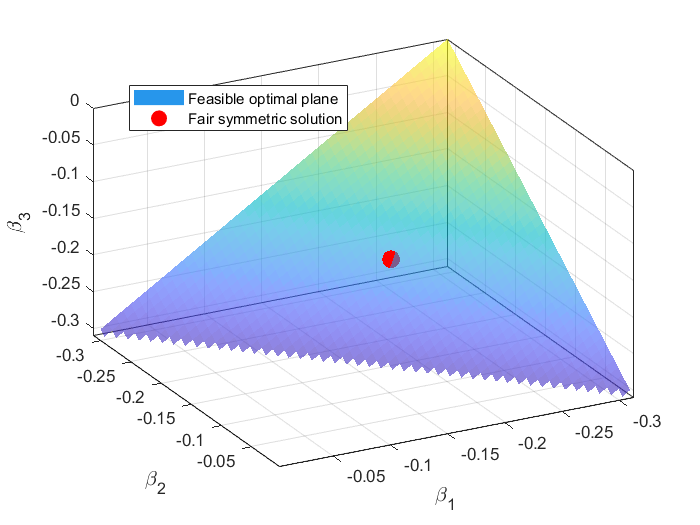
\includegraphics[width=1\linewidth]{figures/risk_seek_sol.png}
    \caption{Feasible risk-seeking Pareto allocations for the example ($n=3$).}
    \label{fig:beta_rs}
\end{figure}

Table~\ref{tab:comparison} and Figures~\ref{fig:algo1_comp_alpha}--\ref{fig:algo1_comp_profit} summarize the performance of all four strategies. The risk-neutral Nash equilibrium incurs a $10.42\%$ profit loss relative to the coalition, while the risk-seeking Pareto-optimal Nash equilibrium fully recovers the coalition-level profit through risk coordination alone, without any change in the game structure. The distributed Algorithm~1 exactly reproduces the centralized Pareto-optimal result: each operator independently estimates $\hat{n}_i=3$ and $\hat{x}_r^o=300$\,MW from the consensus protocols, computes $\beta_i'=-\frac{1}{6}$, and submits the same bids and achieves the same profit as the centralized symmetric Pareto case.

\begin{table}[hbt!]
\centering
\caption{Performance Comparison of Bidding Strategies ($n=3$)}
\label{tab:comparison}
\resizebox{\columnwidth}{!}{%
\begin{tabular}{lcccc}
\hline
Strategy & $\boldsymbol{\alpha}^*$ & $f$ & $g$\,(MW$^2$) & $\sum_i\Pi_i$\,(\$/hr) \\
\hline
Coalition       & $(0.50,\;0.50,\;0.50)$ & $0.50$ & $22{,}500$ & $10{,}800$ \\
RN Nash         & $(0.63,\;0.75,\;0.94)$ & $0.75$ & $16{,}875$ & $\phantom{0}9{,}675$ \\
RS Pareto Nash  & $(0.42,\;0.50,\;0.63)$ & $0.50$ & $22{,}500$ & $10{,}800$ \\
Algo.~1 (Dist.) & $(0.42,\;0.50,\;0.63)$ & $0.50$ & $22{,}500$ & $10{,}800$ \\
\hline
\end{tabular}}
\end{table}

\begin{figure}[hbt!]
    \centering
    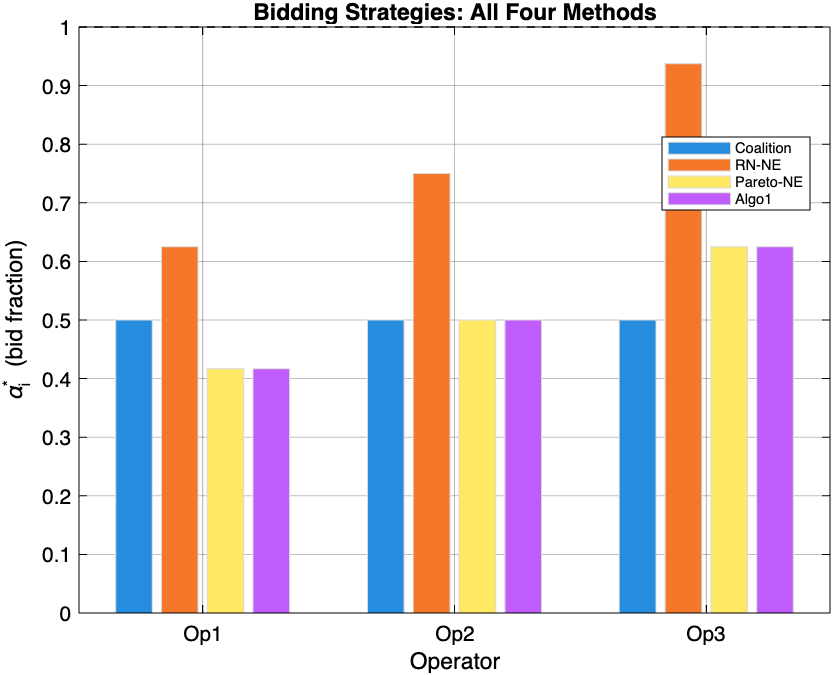
\includegraphics[width=1\linewidth]{figures/algorithm1_comp_alpha_s1.png}
    \caption{Bidding strategies $\alpha_i^*$ for all four strategies.}
    \label{fig:algo1_comp_alpha}
\end{figure}

Figure~\ref{fig:algo1_comp_alpha} shows that the risk-neutral Nash bids are noticeably more aggressive — particularly for Op~3, whose small capacity share ($\eta_3=0.267$) drives $\alpha_3^*$ close to~1. Risk-seeking Pareto coordination uniformly lowers and rebalances the bids toward the coalition optimum, with Algorithm~1 exactly reproducing the centralized result.

\begin{figure}[hbt!]
    \centering
    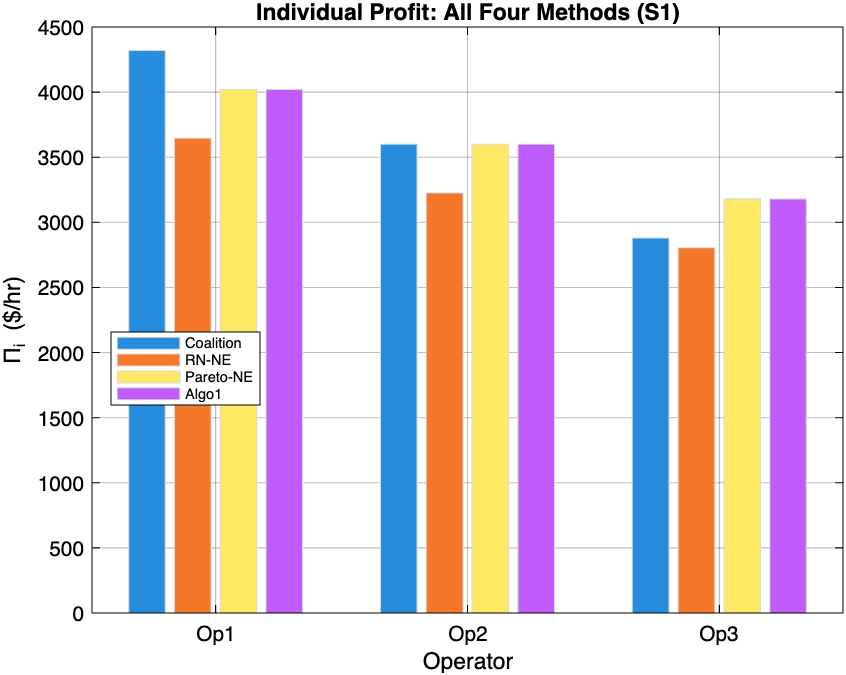
\includegraphics[width=1\linewidth]{figures/algorithm1_comp_profit_s1.png}
    \caption{Individual profits $\Pi_i$ for all four strategies (Scenario~1).}
    \label{fig:algo1_comp_profit}
\end{figure}

\begin{figure}[hbt!]
    \centering
    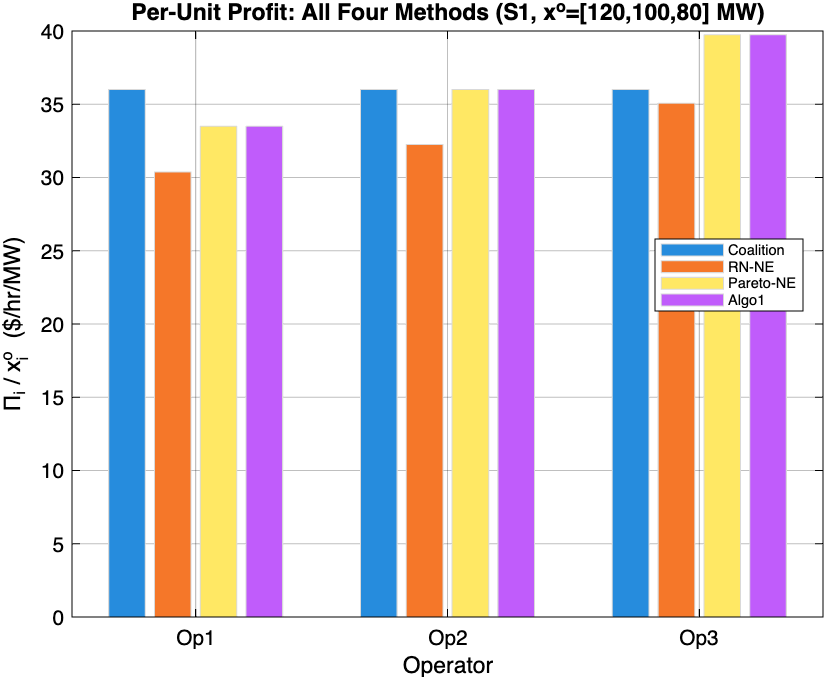
\includegraphics[width=1\linewidth]{figures/algorithm1_comp_profit_perunit_s1.png}
    \caption{Per-unit profit $\Pi_i/x_i^o$ (\$/hr/MW) for all four strategies (Scenario~1). Normalizing by capacity reveals that smaller operators earn disproportionately less per MW under risk-neutral Nash; Pareto coordination through risk-seeking equalizes the per-unit returns across operators.}
    \label{fig:algo1_comp_profit_perunit_s1}
\end{figure}

Figure~\ref{fig:algo1_comp_profit} confirms that the profit improvement under Pareto coordination is shared across all operators: each $\Pi_i$ rises relative to the risk-neutral Nash case, so the move from RN to RS is a Pareto improvement in the game-theoretic sense — no operator is made worse off by adopting the risk-seeking strategy. Figure~\ref{fig:algo1_comp_profit_perunit_s1} further shows the per-unit perspective: under risk-neutral Nash, the smaller Op~3 earns less per MW of installed capacity, while Pareto coordination through risk-seeking restores equal per-unit returns.

\subsection{Heterogeneous Pareto Risk Allocations}

Theorem~2 states that any $\boldsymbol{\beta}$ satisfying $\sum_i\beta_i' = (1-n)/4$ achieves Pareto optimality, yielding infinitely many valid heterogeneous allocations. Three representative allocations for the base parameters illustrate this flexibility:
\begin{itemize}
    \item \textbf{Symmetric ERS}: $\beta_i'=-\frac{1}{6}$ for all $i$ (Corollary~5a). Bids are $\boldsymbol{\alpha}^*=(0.417,\,0.500,\,0.625)$, $f=0.5$, $g=g^{\max}$.
    \item \textbf{Hetero~A}: $\boldsymbol{\beta}'=(-0.10,\,-0.17,\,-0.23)$ — Op~3 (smallest share) is most risk-seeking. Bids become $\boldsymbol{\alpha}^*=(0.750,\,0.480,\,0.150)$, with $f=0.5$ and $g=g^{\max}$ fully preserved.
    \item \textbf{Hetero~B}: $\boldsymbol{\beta}'=(-0.23,\,-0.17,\,-0.10)$ — Op~1 is most risk-seeking. Although $\sum_i\beta_i'=-0.5$ satisfies the Pareto aggregate condition, Op~3's low risk tolerance yields $\alpha_3^*\approx1.12>1$, violating the capacity constraint. Clamping reduces $f$ below $\frac{1}{2}$ and incurs an efficiency loss.
\end{itemize}

Symmetric ERS and Hetero~A both achieve $\Pi^{\rm total}=10{,}800$\,\$/hr, but distribute profits differently: Hetero~A shifts profit toward Op~1 (higher bid) and away from Op~3 (lower bid). This gives a regulator or cooperative agreement a mechanism to adjust equity without sacrificing aggregate efficiency — a direct consequence of the infinite-solution structure of Theorem~2.

\subsection{Overbidding Impact}

From~\eqref{eq:overbid_bound}, overbidding occurs for operator~$i$ at the ERS optimum whenever $\eta_i < \frac{1}{2n}$. For the original parameters in Table~\ref{tab:example_params}, $\eta_i \in \{0.40, 0.33, 0.27\}$ all exceed $\frac{1}{6}$, so $\Omega_{\rm ERS}=\varnothing$ and no overbidding occurs; Scenario~1 in Table~\ref{tab:overbid_compare} confirms that the symmetric Pareto allocation $\beta'^* = -\frac{1}{6}$ achieves $f=0.5$ and $g=g^{\max}$.

To illustrate the heterogeneous-$\beta$ branch of Corollary~5b, we introduce \textit{Scenario~2} by setting $x_3^o = 30$\,MW, giving $x_r^o = 250$\,MW and $\boldsymbol{\eta}=(0.48,\,0.40,\,0.12)$. Operator~3 has $\eta_3 < \tfrac{1}{2n}=\tfrac{1}{6}$, so $\Omega_{\rm ERS}=\{3\}$ and the homogeneous ERS bid is $\alpha_3^*=\tfrac{1}{2n\eta_3}\approx1.39>1$.

The partition~\eqref{eq:partition_Omega} gives $\eta_{\max}=0.48$, $\eta_{\min}=0.12$, midpoint $\eta_c=0.30$, hence $\Omega=\{1,2\}$ and $\Omega^c=\{3\}$. Substituting into~\eqref{eq:beta_hetero}--\eqref{eq:alpha_hetero} with $\sum_{j\in\Omega}\eta_j=0.88$, $\sum_{j\in\Omega^c}\eta_j=0.12$, $|\Omega|=2$:
\begin{align}
  4a_2\beta_3^* &= 2\eta_3-1 = -0.76,\qquad \alpha_3^*=1,\notag\\
  4a_2\beta_{1,2}^* &= \tfrac{0.88-0.12}{2}-1 = -0.62, \notag\\
  \alpha_1^* &= \tfrac{0.76}{4\cdot 0.48}\approx 0.396, \qquad
  \alpha_2^* = \tfrac{0.76}{4\cdot 0.40}=0.475, \notag
\end{align}
yielding $\boldsymbol{\alpha}^*=(0.396,\,0.475,\,1.000)$, $f=0.500$, and $g=g^{\max}=15{,}625$\,MW$^2$. The construction is one-shot: the partition is read off directly from $(\eta_{\max},\eta_{\min})$, no iterative saturation check is needed.

\begin{table}[hbt!]
\centering
\caption{Overbidding Scenario Comparison ($n=3$, $a_2=0.1$, $x_L^o=400$\,MW)}
\label{tab:overbid_compare}
\resizebox{\columnwidth}{!}{%
\setlength{\tabcolsep}{4pt}
\begin{tabular}{lccccccccc}
\hline
Scenario & $\Omega^c$ & $4a_2\beta_i^*$ & $\alpha_1^*$ & $\alpha_2^*$ & $\alpha_3^*$ & $f$ & $g$\,(MW$^2$) & $\sum\Pi_i$\,(\$/hr) & loss \\
\hline
S1: original (no overbid)         & $\varnothing$ & $-2/3$ (sym.)         & $0.417$ & $0.500$ & $0.625$ & $0.500$ & $22{,}500$ & $10{,}800$ & $0\%$ \\
S2: unclamped sym.\ ERS           & $\{3\}$       & $-2/3$ (sym.)         & $0.347$ & $0.417$ & $1.389$ & $0.500$ & $15{,}625$ & $10{,}875$ & $0\%$ \\
S2: hetero-$\beta$ (Cor.~5b)      & $\{3\}$       & $(-0.62,-0.62,-0.76)$ & $0.396$ & $0.475$ & $1.000$ & $0.500$ & $15{,}625$ & $10{,}875$ & $0\%$ \\
S3: unclamped sym.\ ERS           & $\{2,3\}$     & $-2/3$ (sym.)         & $0.238$ & $1.111$ & $1.111$ & $0.500$ & $22{,}500$ & $10{,}800$ & $0\%$ \\
S3: hetero-$\beta$ (Cor.~5b)      & $\{2,3\}$     & $(-0.60,-0.70,-0.70)$ & $0.286$ & $1.000$ & $1.000$ & $0.500$ & $22{,}500$ & $10{,}800$ & $0\%$ \\
\hline
\multicolumn{10}{l}{S2: $x_3^o{=}30$\,MW, $x_r^o{=}250$\,MW;\quad S3: $x^o{=}(210,45,45)$\,MW, $x_r^o{=}300$\,MW; loss $= g^{\max}$ gap.}
\end{tabular}}
\end{table}

\begin{table}[hbt!]
\centering
\caption{ERS Strategy Performance Under Overbidding Scenarios ($n=3$, $a_2=0.1$, $x_L^o=400$\,MW)}
\label{tab:ers_compare}
\resizebox{\columnwidth}{!}{%
\begin{tabular}{llcccc}
\hline
Scenario & Strategy & $\boldsymbol{\alpha}^*$ & $f$ & $g$\,(MW$^2$) & $\sum_i\Pi_i$\,(\$/hr) \\
\hline
\multirow{4}{*}{S2 ($x_r^o{=}250$\,MW)} &
  Coalition         & $(0.500,\;0.500,\;0.500)$ & $0.500$ & $15{,}625$ & $10{,}875$ \\
& RN Nash           & $(0.521,\;0.625,\;2.083)$ & $0.750$ & $11{,}719$ & $10{,}094$ \\
& Pareto-NE         & $(0.347,\;0.417,\;1.389)$ & $0.500$ & $15{,}625$ & $10{,}875$ \\
& Algo.~1 (Cor.~5b) & $(0.396,\;0.475,\;1.000)$ & $0.500$ & $15{,}625$ & $10{,}875$ \\
\hline
\multirow{4}{*}{S3 ($x_r^o{=}300$\,MW)} &
  Coalition         & $(0.500,\;0.500,\;0.500)$ & $0.500$ & $22{,}500$ & $10{,}800$ \\
& RN Nash           & $(0.357,\;1.667,\;1.667)$ & $0.750$ & $16{,}875$ & $\phantom{0}9{,}675$ \\
& Pareto-NE         & $(0.238,\;1.111,\;1.111)$ & $0.500$ & $22{,}500$ & $10{,}800$ \\
& Algo.~1 (Cor.~5b) & $(0.286,\;1.000,\;1.000)$ & $0.500$ & $22{,}500$ & $10{,}800$ \\
\hline
\multicolumn{6}{l}{Pareto-NE bids in italics are infeasible ($\alpha_i>1$); Algo.~1 enforces feasibility via Cor.~5b.}
\end{tabular}}
\end{table}

Table~\ref{tab:ers_compare} summarizes the four primary strategies across Scenarios~2 and~3, confirming that Algorithm~1 matches the Coalition and Pareto-NE aggregate performance while enforcing feasibility. Figure~\ref{fig:algo1_overbid_alpha} applies all six strategies to Scenario~2 ($x_3^o=30$\,MW, $\eta_3=0.12$), the same capacity configuration examined analytically above. Under these parameters, $\eta_3 < \tfrac{1}{2n} = \tfrac{1}{6}$, so the unconstrained symmetric Pareto bid for Op~3 is $\alpha_3^* = \tfrac{1}{6\eta_3} \approx 1.39 > 1$ — a feasibility violation. The risk-neutral Nash equilibrium is even more aggressive ($\alpha_3^* \approx 2.08$). Algorithm~1 follows the heterogeneous-$\beta$ branch of Corollary~5b: it identifies the partition $\Omega=\{1,2\}$, $\Omega^c=\{3\}$ via max-/min-consensus, recovers $\sum_{j\in\Omega}\eta_j-\sum_{j\in\Omega^c}\eta_j=0.76$ and $|\Omega|=2$ from two short auxiliary consensus rounds, and submits $(0.396,\,0.475,\,1.000)$ — landing the Algo~1 bar \emph{exactly} at the $\alpha=1$ boundary while recovering $f=\frac{1}{2}$. Also shown is a heterogeneous-$\beta$ deviation scenario ($\beta'=[{-0.20},{-0.15},{-0.05}]$, ``Unclamped OB'') and its naive per-operator clamp (``No-overbid''), which can push Op~3 far above~1 without the principled risk re-allocation that Algo~1 performs.

\begin{figure}[hbt!]
    \centering
    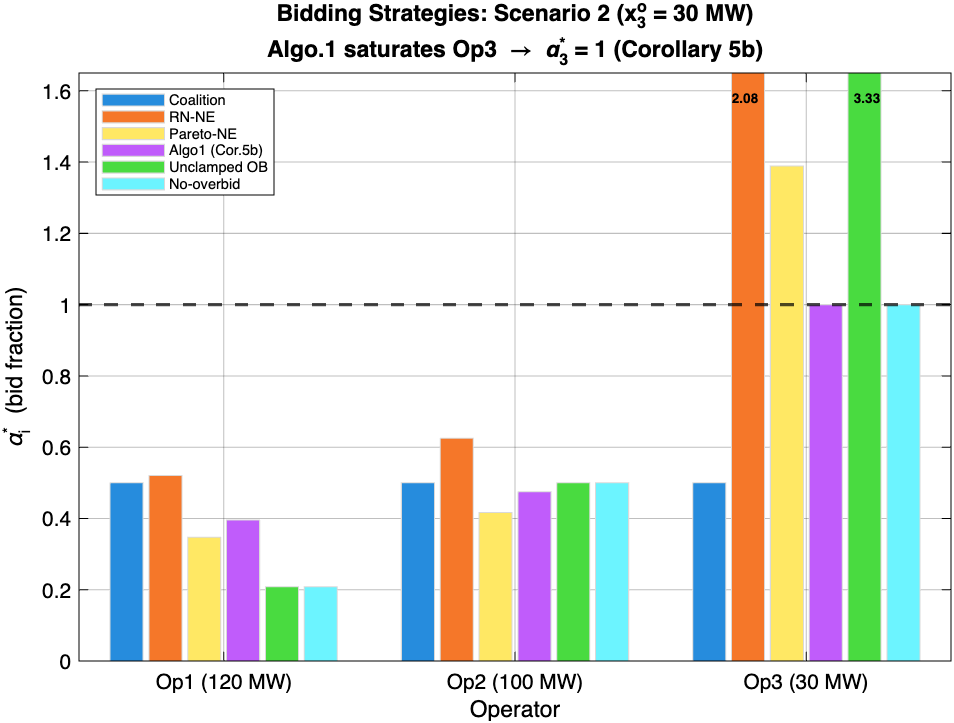
\includegraphics[width=1\linewidth]{figures/algorithm1_overbid_alpha_s2.png}
    \caption{Bidding strategies $\alpha_i^*$ under Scenario~2 ($x_3^o=30$\,MW). The dashed line marks $\alpha=1$; both the unconstrained Pareto-NE and RN-NE overbid at Op~3, while Algorithm~1 (Corollary~5b saturation branch) places $\alpha_3^*$ exactly at~1. Bars for RN-NE and Unclamped~OB at Op~3 extend beyond the $y$-axis clip; their values are annotated.}
    \label{fig:algo1_overbid_alpha}
\end{figure}

Figures~\ref{fig:algo1_overbid_profit} and~\ref{fig:algo1_overbid_profit_perunit} show the profit consequences under Scenario~2. Coalition and Algo~1 achieve the same total profit ($f=0.5$, $g=g^{\max}=15{,}625$\,MW$^2$), with Op~3 receiving a smaller absolute share due to its reduced capacity. Pareto-NE produces the same aggregate outcome analytically but is infeasible ($\alpha_3^*>1$). Unclamped overbidding overshoots $f=0.5$, reducing aggregate efficiency, while the simple per-operator clamp partially recovers it without restoring the Pareto target.

\begin{figure}[hbt!]
    \centering
    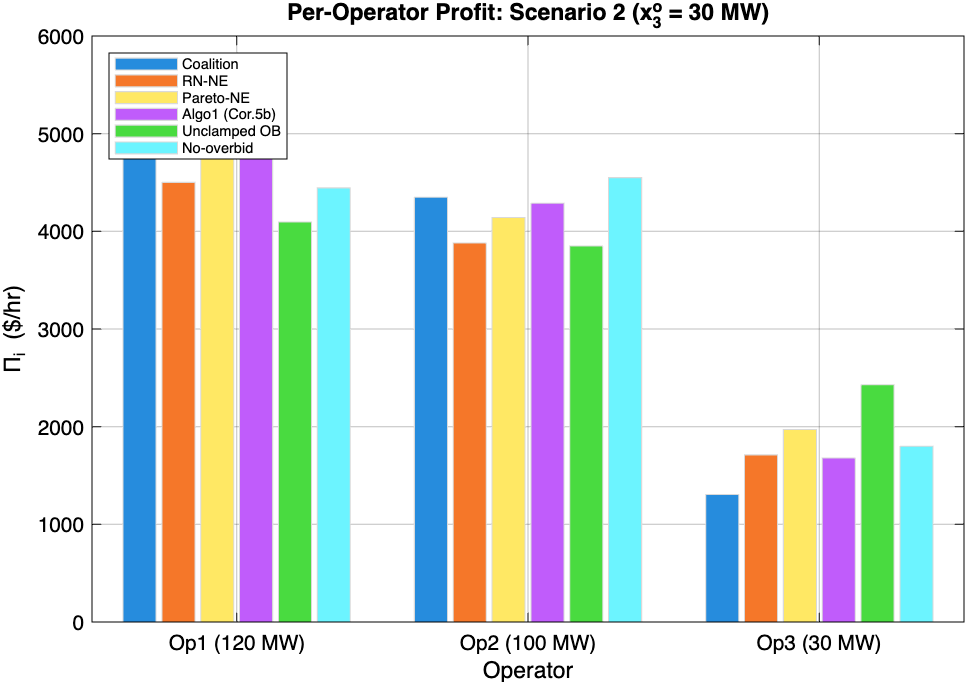
\includegraphics[width=1\linewidth]{figures/algorithm1_overbid_profit_s2.png}
    \caption{Per-operator profit $\Pi_i$ under Scenario~2 for all six strategies. Coalition and Algo~1 achieve the same total profit at $f=0.5$; risk-neutral and unclamped strategies overshoot $f=\tfrac{1}{2}$, reducing aggregate efficiency.}
    \label{fig:algo1_overbid_profit}
\end{figure}

\begin{figure}[hbt!]
    \centering
    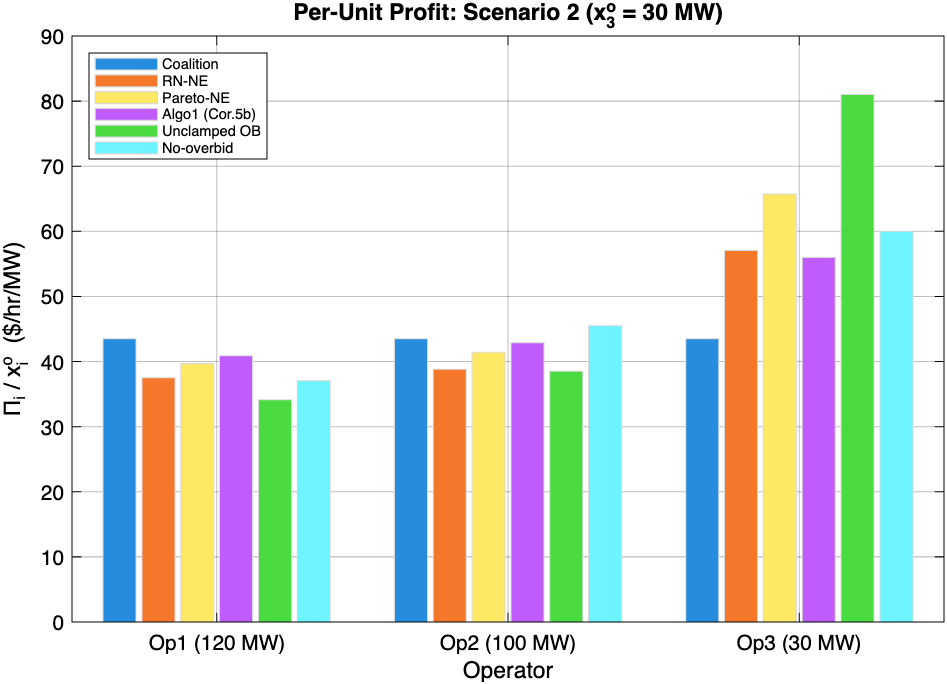
\includegraphics[width=1\linewidth]{figures/algorithm1_overbid_profit_perunit_s2.png}
    \caption{Per-unit profit $\Pi_i/x_i^o$ under Scenario~2. Algorithm~1 achieves per-unit equity comparable to the Coalition benchmark; unclamped overbidding distorts Op~3's per-unit revenue upward at the expense of the other operators.}
    \label{fig:algo1_overbid_profit_perunit}
\end{figure}

\noindent\textbf{Observation.} \textit{Overbidding at the ERS optimum is not an artifact of deviating from the Pareto sum condition, but a structural consequence of small renewable share: operator~$i$ overbids whenever $\eta_i < \frac{1}{2n}$, regardless of the chosen common $\beta'$. No homogeneous-$\beta$ policy can simultaneously achieve feasibility and $f=\tfrac12$. The heterogeneous allocation of Corollary~5b assigns a more risk-seeking $\beta_i^*$ to capacity-limited operators (driving $\alpha_i^*=1$ exactly) and a common, milder $\beta_i^*$ to the remainder (restoring $f=\tfrac12$), recovering $g^{\max}$ with no efficiency penalty.}


\subsection{Constrained Risk-Neutral Nash (Corollary~4)}

To isolate the value of risk coordination under capacity constraints, consider Scenario~2 capacities ($x_3^o=30$\,MW, $x_r^o=250$\,MW) with all operators risk-neutral ($\beta_i=0$) and overbidding forbidden. Since $\eta_3=0.12<\frac{1}{n+1}=0.25$, Corollary~4 applies with $\Omega_{\rm RN}=\{3\}$. Op~3 is clamped to $\alpha_3^*=1$ and the remaining operators are re-solved:
\[
    \alpha_i^* = \frac{1-\sum_{j\in\Omega_{\rm RN}}\eta_j}{(n+1-|\Omega_{\rm RN}|)\,\eta_i}
    = \frac{0.88}{3\eta_i}, \quad i\in\{1,2\},
\]
yielding $\boldsymbol{\alpha}^*=(0.611,\,0.733,\,1.000)$, $f=0.707$, and $g\approx12{,}946$\,MW$^2$.

Figure~\ref{fig:cor4_alpha} compares the three strategies for Scenario~2. The unconstrained RN naturally drives Op~3 to $\alpha_3^*\approx2.08$ (overbidding); Corollary~4 enforces feasibility by re-solving the equilibrium, but $f=0.707\gg\frac{1}{2}$ leaves market efficiency at only ${\approx}83\%$ of $g^{\max}=15{,}625$\,MW$^2$. This quantifies the efficiency cost of foregoing risk coordination: even when overbidding is eliminated, risk-neutral operation incurs a persistent market efficiency loss that risk-seeking coordination avoids.

\begin{figure}[hbt!]
    \centering
    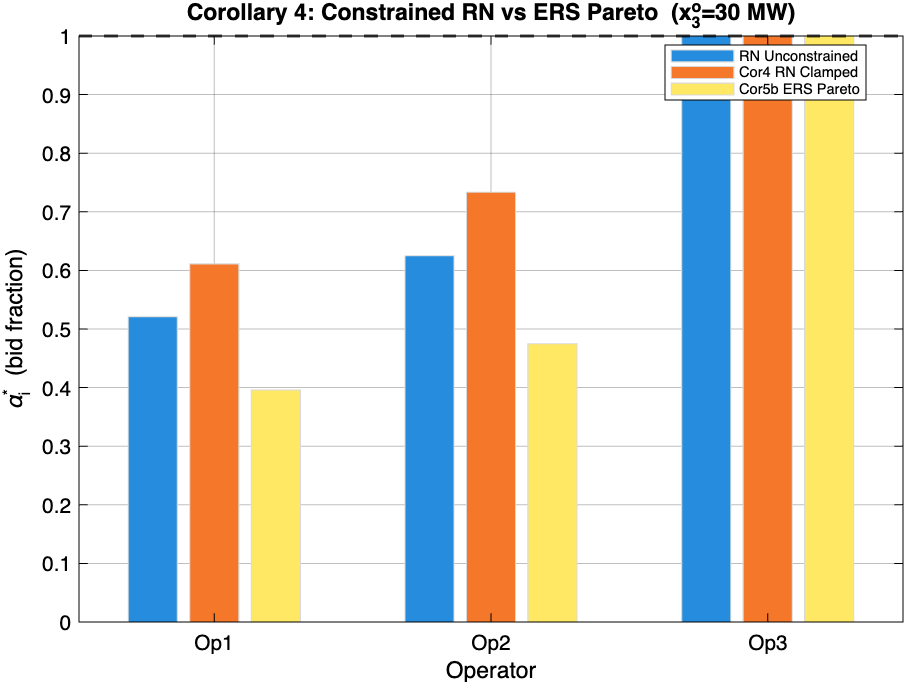
\includegraphics[width=1\linewidth]{figures/cor4_constrained_rn_alpha.png}
    \caption{Corollary~4: bidding strategies under unconstrained RN and constrained RN (Cor.~4 clamped) for Scenario~2 ($x_3^o=30$\,MW). Constrained RN enforces feasibility but leaves $f=0.707\gg\frac{1}{2}$, incurring a persistent efficiency loss relative to risk-seeking coordination.}
    \label{fig:cor4_alpha}
\end{figure}

\subsection{Multiple Operator Saturation (Corollary~5b)}

To validate the generality of Corollary~5b beyond $|\Omega^c|=1$, we introduce \textit{Scenario~3} by setting $x^o=(210,45,45)$\,MW giving $\eta=(0.70,0.15,0.15)$.  The unconstrained ERS formula yields $\alpha_{2,3}^*\approx1.11>1$, so Ops~2 and~3 would overbid; the heterogeneous-$\beta$ construction of Corollary~5b corrects this.

With $\eta_{\max}=0.70$ and $\eta_{\min}=0.15$, the cutoff and partition are
\[
    \eta_c = \tfrac{1}{2}(0.70+0.15) = 0.425,
    \qquad \Omega=\{1\},\quad \Omega^c=\{2,3\}.
\]
We have $\sum_{j\in\Omega}\eta_j=0.70$, $\sum_{j\in\Omega^c}\eta_j=0.30$, so $D\triangleq\sum_{j\in\Omega}\eta_j-\sum_{j\in\Omega^c}\eta_j=0.40$ and $|\Omega|=1$.
Substituting into \eqref{eq:alpha_hetero}:
\[
    \alpha_1^* = \frac{D}{2\,|\Omega|\,\eta_1}
               = \frac{0.40}{2\times0.70} = \frac{2}{7}\approx0.286,
    \qquad \alpha_2^*=\alpha_3^*=1.
\]
One can verify $f=\tfrac{2}{7}\times0.70+1\times0.15+1\times0.15=0.500$ and $g=g_{\max}=22{,}500$\,MW$^2$, achieving the full Pareto optimum even with two saturating operators.  This contrasts sharply with a na\"{i}ve homogeneous-$\beta_0$ approach, which would give $f=0.825$ and $g\approx13{,}001$\,MW$^2$ — confirming that the heterogeneous construction eliminates the efficiency penalty regardless of $|\Omega^c|$.

Figure~\ref{fig:algo1_overbid_alpha_s3} compares all six strategies under Scenario~3. Both RN-NE and the unconstrained Pareto-NE overbid at Ops~2 and~3, while Algorithm~1 (Corollary~5b) sets $\alpha_{2,3}^*=1$ exactly and recovers $f=\frac{1}{2}$ without the efficiency penalty incurred by naive clamping. Figures~\ref{fig:algo1_overbid_profit_s3} and~\ref{fig:algo1_overbid_profit_perunit_s3} show the corresponding per-operator and per-unit profits.

\begin{figure}[hbt!]
    \centering
    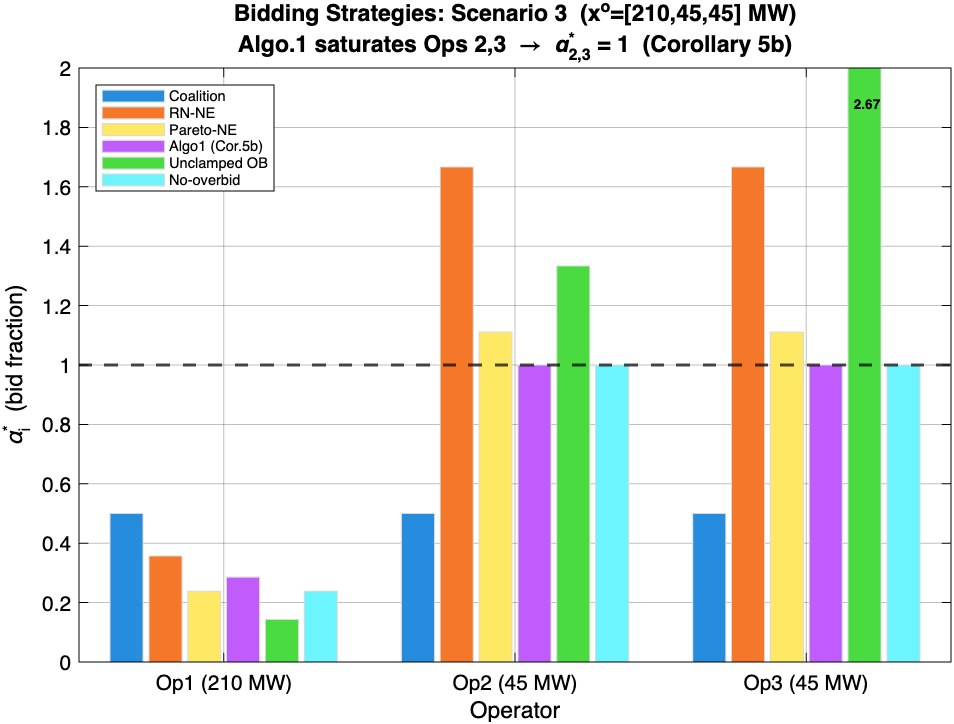
\includegraphics[width=1\linewidth]{figures/algorithm1_overbid_alpha_s3.png}
    \caption{Bidding strategies under Scenario~3 ($x^o=(210,45,45)$\,MW). Both RN-NE and Pareto-NE overbid at Ops~2 and~3; Algorithm~1 (Cor.~5b) places $\alpha_{2,3}^*$ exactly at~1. Naive clamping reduces $f$ below $\tfrac{1}{2}$.}
    \label{fig:algo1_overbid_alpha_s3}
\end{figure}

\begin{figure}[hbt!]
    \centering
    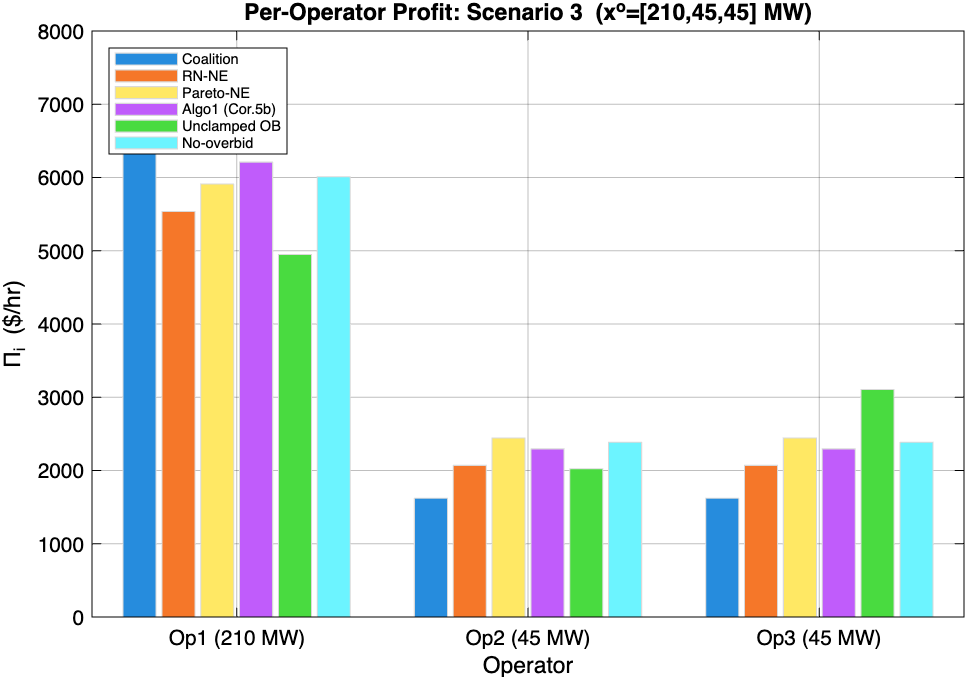
\includegraphics[width=1\linewidth]{figures/algorithm1_overbid_profit_s3.png}
    \caption{Per-operator profit $\Pi_i$ under Scenario~3 for all six strategies. Coalition and Algo~1 both achieve $\sum\Pi_i=10{,}800$\,\$/hr at $f=0.5$; risk-neutral and unclamped strategies reduce aggregate efficiency.}
    \label{fig:algo1_overbid_profit_s3}
\end{figure}

\begin{figure}[hbt!]
    \centering
    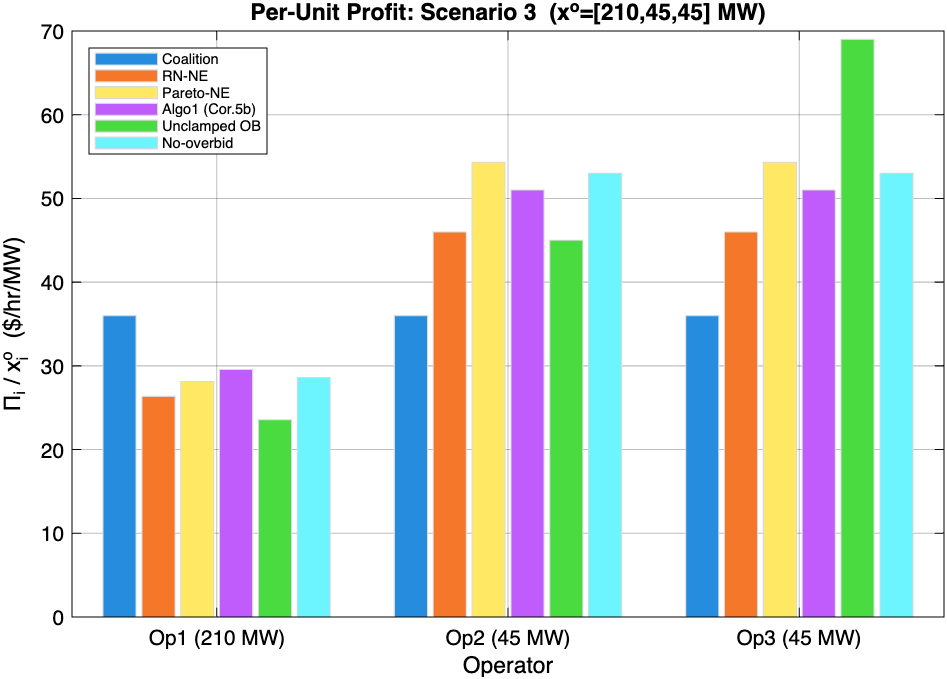
\includegraphics[width=1\linewidth]{figures/algorithm1_overbid_profit_perunit_s3.png}
    \caption{Per-unit profit $\Pi_i/x_i^o$ under Scenario~3. Algorithm~1 restores per-unit equity comparable to the Coalition benchmark.}
    \label{fig:algo1_overbid_profit_perunit_s3}
\end{figure}

\subsection{Solutions under Distributed Algorithms}

Figures~\ref{fig:algo1_xi}--\ref{fig:algo1_psi} show convergence of the consensus states. The initial conditions follow Algorithm~\ref{alg:dist_risk_aware}: the utility sets $\xi_4(0)=1$, $\psi_4(0)=0$; each operator sets $\xi_i(0)=0$, $\psi_i(0)=x_i^o$. All agents converge to the common average $\xi_i(k)\to\frac{1}{4}$ and $\psi_i(k)\to\frac{x_r^o}{4}=75$\,MW. From these converged values, each operator~$i$ locally computes the quantities shown in Table~\ref{tab:algo1_computed}, confirming that every operator independently recovers the correct $\hat{n}_i=3$, $\eta_i$, and $\beta_i'=-\frac{1}{6}$ without any additional communication.

\begin{figure}[hbt!]
    \centering
    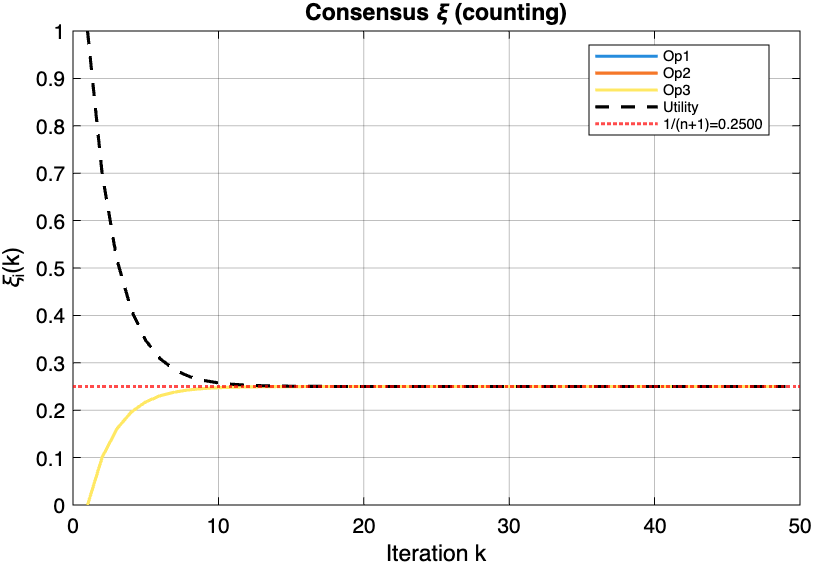
\includegraphics[width=1\linewidth]{figures/algorithm1_xi_consensus.png}
    \caption{Algorithm~1 consensus trajectory for $\xi_i$.}
    \label{fig:algo1_xi}
\end{figure}

\begin{figure}[hbt!]
    \centering
    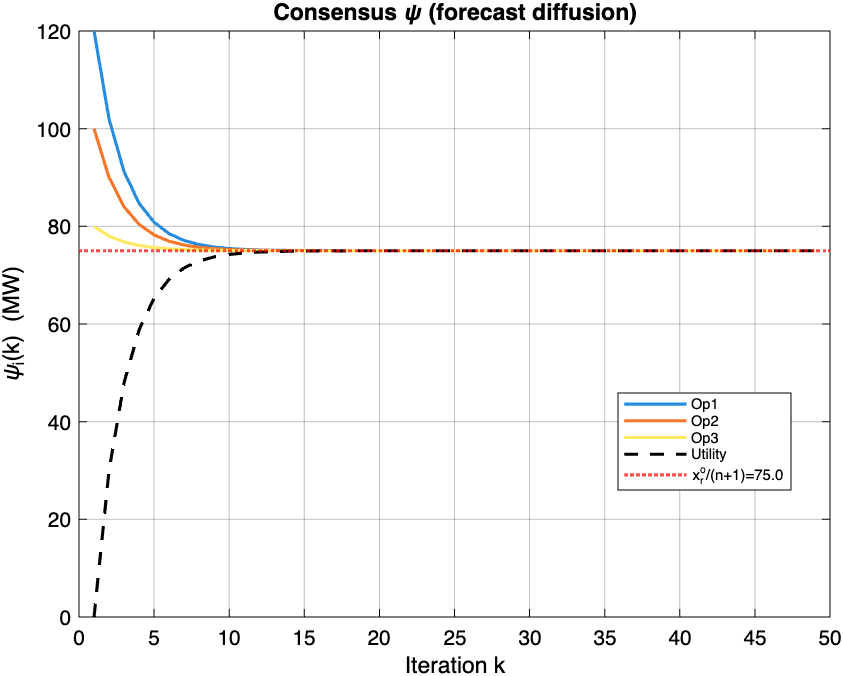
\includegraphics[width=1\linewidth]{figures/algorithm1_psi_consensus.png}
    \caption{Algorithm~1 consensus trajectory for $\psi_i$.}
    \label{fig:algo1_psi}
\end{figure}

\begin{table}[hbt!]
\centering
\caption{Quantities computed locally by each operator after consensus convergence}
\label{tab:algo1_computed}
\begin{tabular}{lcccc}
\hline
Op. & $\xi_i^\infty$ & $\hat{n}_i $ & $\eta_i$ & $\beta_i'$ \\
\hline
1 & 0.25 & 3 & $2/5$ & $-1/6$ \\
2 & 0.25 & 3 & $1/3$ & $-1/6$ \\
3 & 0.25 & 3 & $4/15$ & $-1/6$ \\
\hline
\end{tabular}
\end{table}
\noindent\textbf{Remark~3.} \textit{The convergence rate of Algorithm~1 on the star graph $K_{1,n}$ is $O(\log(1/\varepsilon))$ per consensus round, independent of the number of operators~$n$. This follows from the algebraic connectivity $\lambda_2(L)=1$ of $K_{1,n}$, which is established in Section~V and does not degrade as $n$ grows.}

The Corollary~5b branch of Algorithm~1 is validated on Scenarios~2 and~3.  In each case operators first run max- and min-consensus on $\eta_i$ to recover $\eta_{\max}$ and $\eta_{\min}$, then each operator locally computes $\eta_c=(\eta_{\max}+\eta_{\min})/2$ and determines its partition membership.  In Scenario~2 ($\eta_c=0.30$): Ops~1 and~2 belong to $\Omega$ and seed $\sigma_i(0)=+\eta_i$, while Op~3 belongs to $\Omega^c$ and seeds $\sigma_3(0)=-0.12$; the indicator seeds are $\mu_{1,2}(0)=1$, $\mu_3(0)=0$.  In Scenario~3 ($\eta_c=0.425$): Op~1 alone belongs to $\Omega$ and seeds $\sigma_1(0)=+0.70$, while Ops~2 and~3 each seed $\sigma_i(0)=-0.15$; the indicator seeds are $\mu_1(0)=1$, $\mu_{2,3}(0)=0$.  In both cases the $\sigma$- and $\mu$-consensus rounds converge and the locally recovered $\widehat{D}=\sum_{j\in\Omega}\eta_j-\sum_{j\in\Omega^c}\eta_j$ and $|\widehat{\Omega}|$ yield bids $\boldsymbol{\alpha}^*$ indistinguishable from the centralized Corollary~5b solution, confirming that partition information is correctly propagated without any central coordinator.

Figures~\ref{fig:sigma_s2}--\ref{fig:sigma_s6} show the $\sigma$-consensus trajectories for Scenarios~2 and~3. Operators in $\Omega$ seed positive values $+\eta_i$ and converge downward; operators in $\Omega^c$ seed negative values $-\eta_i$ and converge upward. The utility (dashed) seeds $\sigma_{n+1}(0)=0$ and rises monotonically to the common steady state. The red dotted line marks the target $D/(n+1)$; dividing by the converged $\xi_i^\infty=1/(n+1)$ recovers $\widehat{D}$ locally at each node.

\begin{figure}[hbt!]
    \centering
    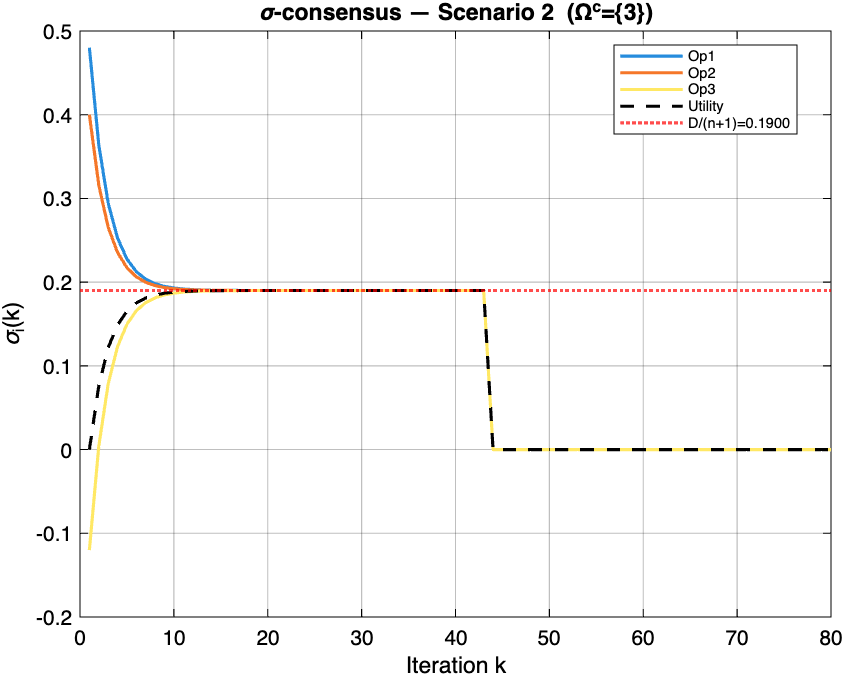
\includegraphics[width=1\linewidth]{figures/sigma_consensus_s2.png}
    \caption{$\sigma$-consensus trajectory for Scenario~2 ($\Omega^c=\{3\}$). Ops~1,2 ($\in\Omega$) seed $+\eta_i$ and converge down; Op~3 ($\in\Omega^c$) seeds $-0.12$ and converges up. The utility (dashed) seeds~$0$ and rises monotonically. Red dotted line: steady-state target $D/(n+1)=0.19$; recovering $\widehat{D}=\sigma_i^\infty/\xi_i^\infty=0.76$.}
    \label{fig:sigma_s2}
\end{figure}

\begin{figure}[hbt!]
    \centering
    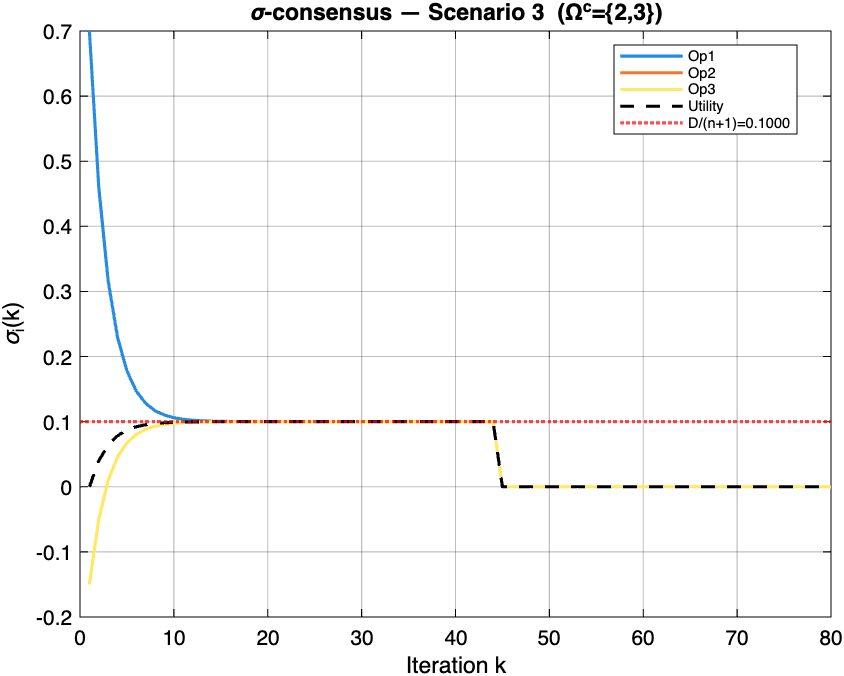
\includegraphics[width=1\linewidth]{figures/sigma_consensus_s6.png}
    \caption{$\sigma$-consensus trajectory for Scenario~3 ($\Omega^c=\{2,3\}$). Op~1 ($\in\Omega$) seeds $+0.70$ and converges down; Ops~2,3 ($\in\Omega^c$) seed $-0.15$ and converge up. The utility (dashed) seeds~$0$ and rises monotonically. Red dotted line: steady-state target $D/(n+1)=0.10$; recovering $\widehat{D}=\sigma_i^\infty/\xi_i^\infty=0.40$.}
    \label{fig:sigma_s6}
\end{figure}

\subsection{Scalability Discussion}

The numerical example above uses $n=3$ operators to keep the exposition concrete. The theoretical results, however, are fully general: Theorems~1--2 and Corollaries~1--5b hold for any $n\geq 1$, and Algorithm~1 requires no modification as $n$ grows. Three structural properties support scalability. First, from Remark~3, the convergence rate of Algorithm~1 is $O(\log(1/\varepsilon))$ per consensus round on the star graph, independent of $n$. Second, each operator performs only local computations (a single division and two multiplications after consensus), so per-operator complexity does not grow with $n$. Third, the overbidding threshold $\eta_i < 1/(2n)$ becomes more stringent as $n$ increases, so in large markets with many similarly-sized operators the unconstrained formula~\eqref{eq:alpha_optimal_simplified} applies without any clamping. Simulation studies at larger scale ($n \in \{10, 50\}$) are deferred to future work, where they will also address sensitivity of the Pareto condition to heterogeneous capacity distributions and transient operator participation.

\begin{comment}

To assess the robustness of the overbidding analysis with respect to initial risk profiles, the outer-loop coordination of $\beta_i'$ is evaluated under six heterogeneous starting points: risk-neutral ($\beta_i'(0)=0$), uniform risk-seeking ($\beta_i'(0)=-1$), uniform risk-averse ($\beta_i'(0)=1$), and three mixed profiles. Figures~\ref{fig:mc_overbid_count} and~\ref{fig:mc_overbid_profit} show the per-operator overbidding indicator and aggregate profit comparison for each case. Operators with smaller capacity shares saturate first in every case, consistent with the threshold ordering of Remark~1. Cases where no operator overbids throughout coordination (e.g., the symmetric Pareto starting point) yield identical unclamped and clamped profit trajectories, while cases with high initial risk-seeking values exhibit a transient profit gap that closes as $\sum\beta_i'$ converges to the Pareto target.

\begin{figure}[hbt!]
    \centering
    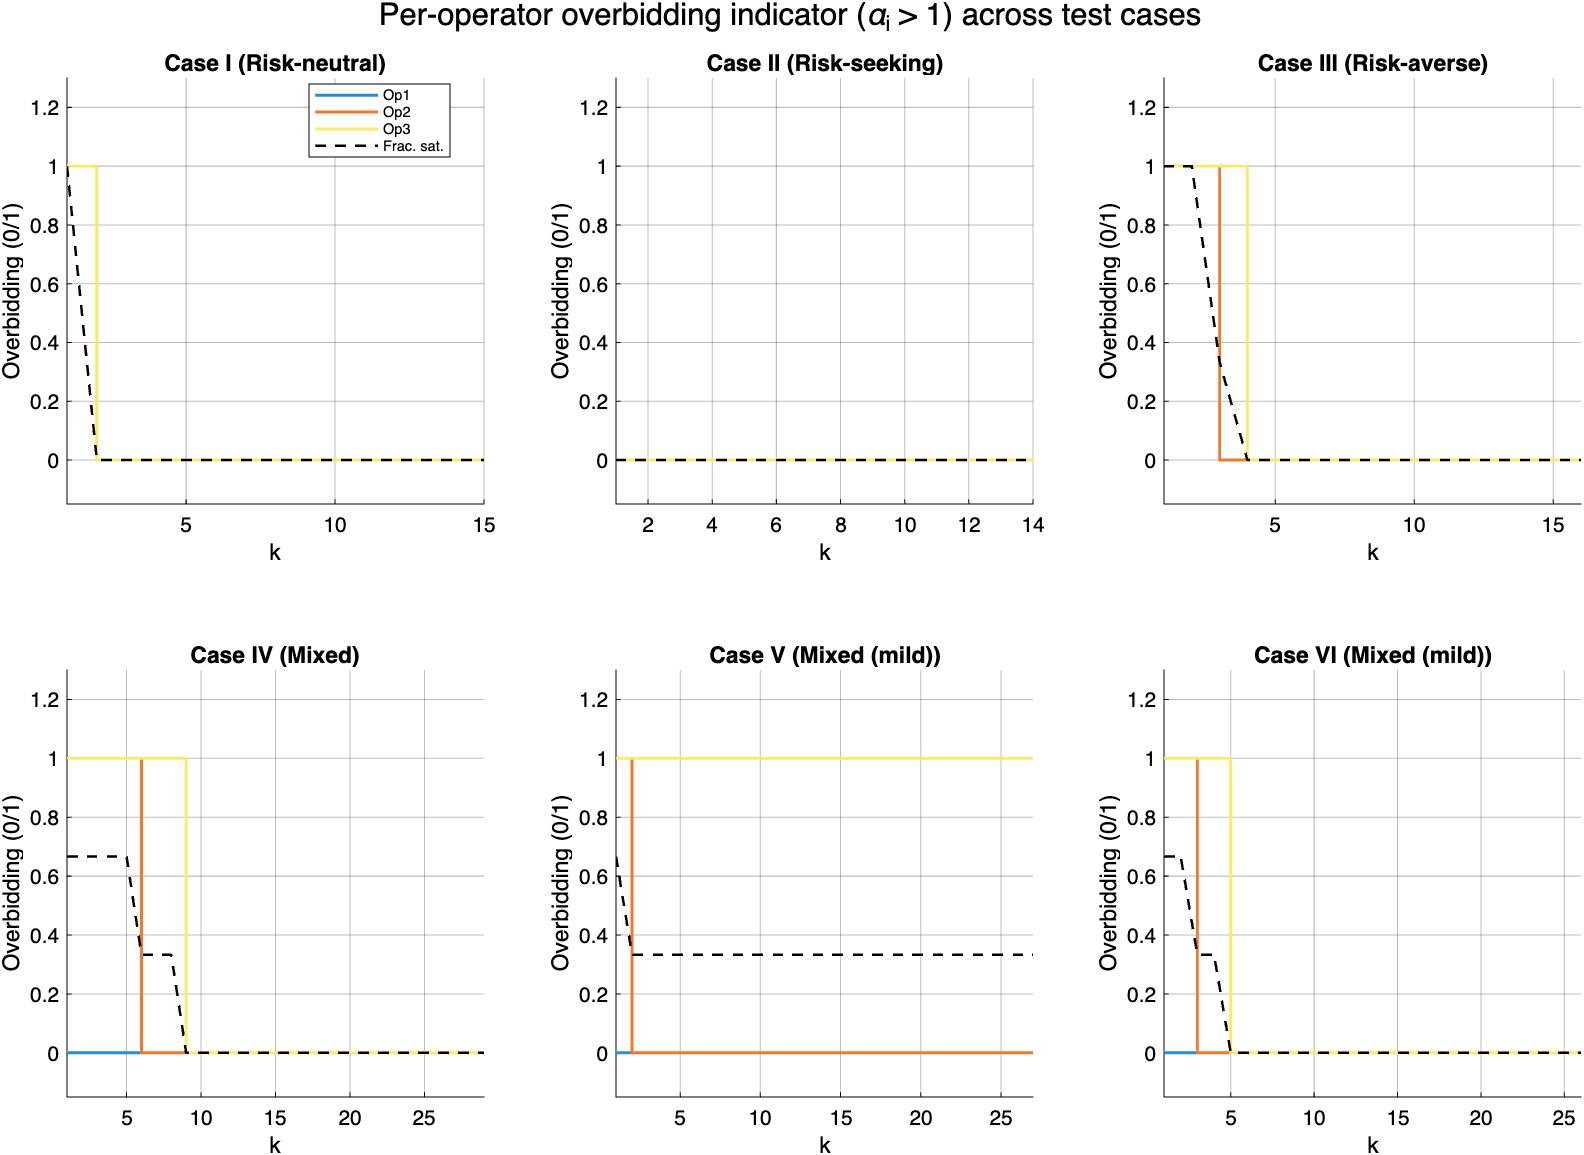
\includegraphics[width=1\linewidth]{figures/mc_overbid_count.png}
    \caption{Per-operator overbidding indicator ($\alpha_i > 1$, shown as 0/1) across six initial risk profiles. Operators with smaller capacity shares ($\eta_i$) saturate earlier in coordination, and the fraction of saturating operators (dashed) confirms the threshold ordering of Remark~1 across all cases.}
    \label{fig:mc_overbid_count}
\end{figure}

\begin{figure}[hbt!]
    \centering
    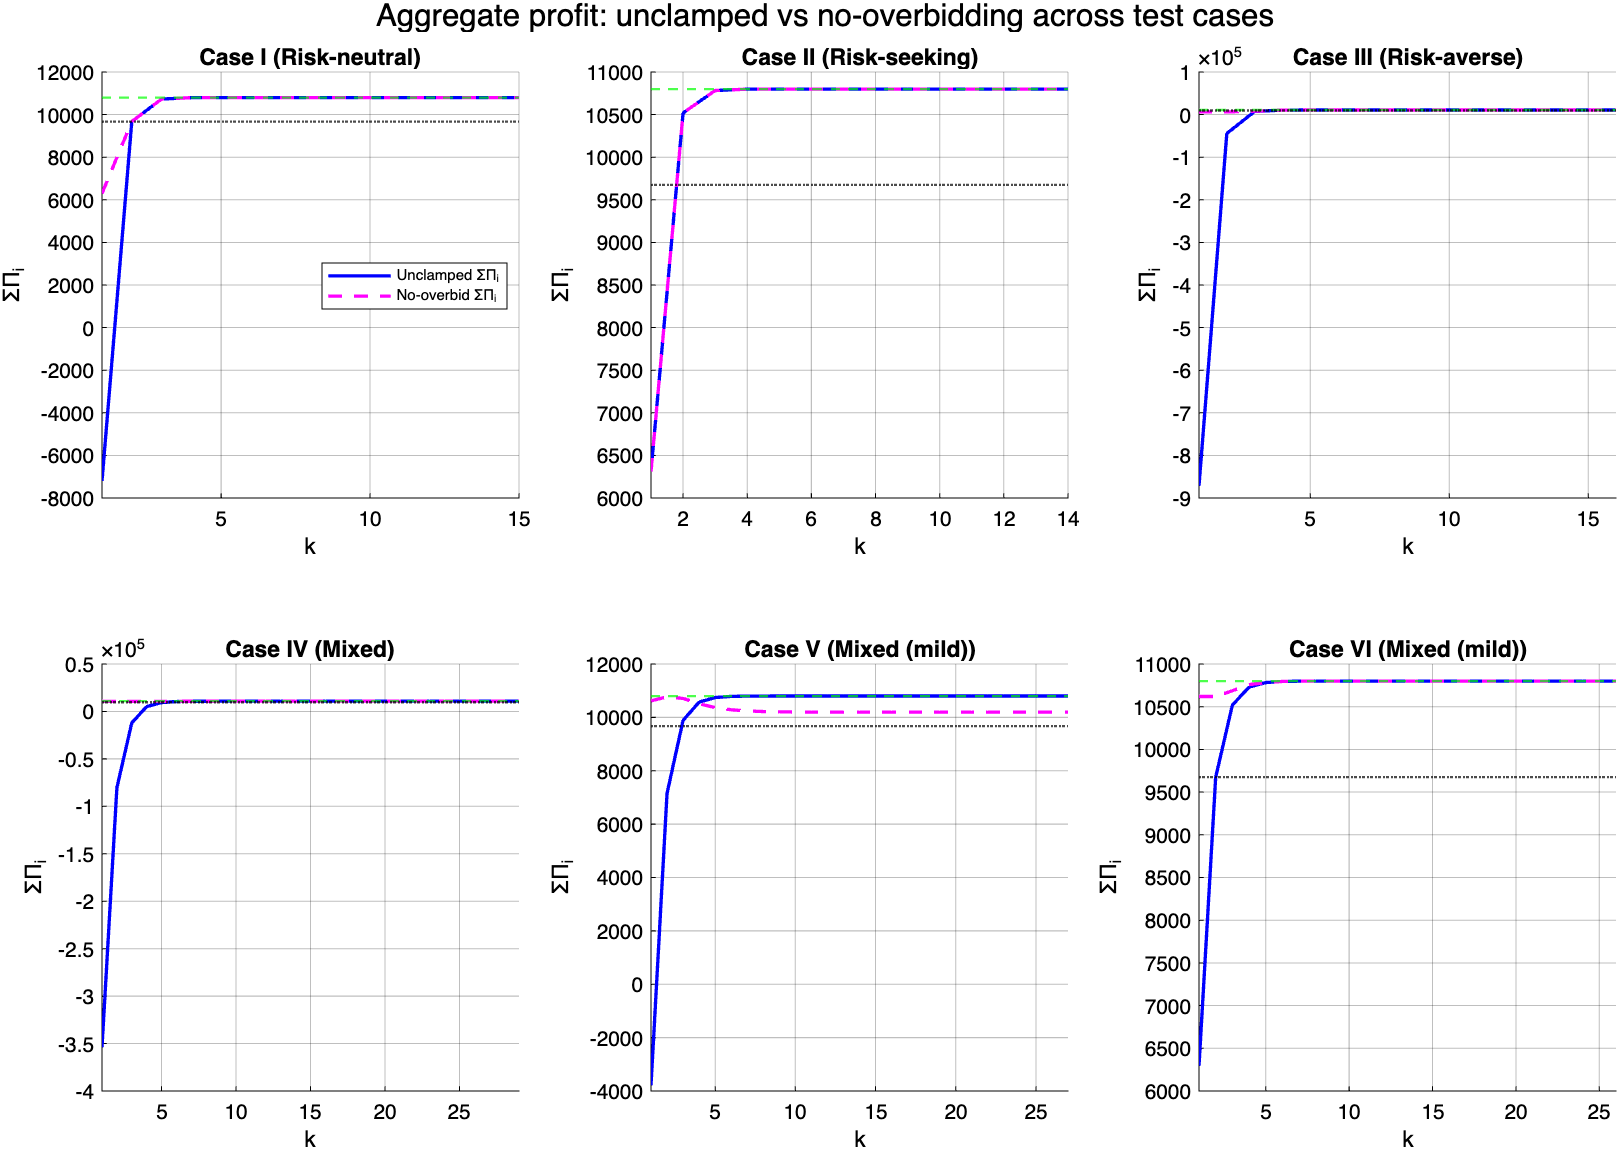
\includegraphics[width=1\linewidth]{figures/mc_overbid_profit.png}
    \caption{Aggregate profit $\sum_i\Pi_i$ under unclamped versus no-overbidding projection across six initial risk profiles. The profit gap is case-dependent and governed by the number of saturating operators; cases with no overbidding show identical trajectories. All cases converge to the Pareto-optimal profit level as coordination proceeds.}
    \label{fig:mc_overbid_profit}
\end{figure}

\end{comment}

\begin{comment}
    

\subsubsection{Algorithm 2: Non-Equal Initial Risk Parameters}
Algorithm~\ref{alg:dist_risk_aware_beta_coord} is evaluated using \texttt{risk\_aware\_power\_system.m} under multiple heterogeneous initial conditions $\beta_i'(0)$. The study focuses on whether distributed coordination of the aggregate risk parameter and unclamped one-shot bidding preserve the Pareto target. Accordingly, bid/profit comparisons are reported in this subsection (after the risk-parameter coordination stage is complete).

\begin{figure}[hbt!]
    \centering
    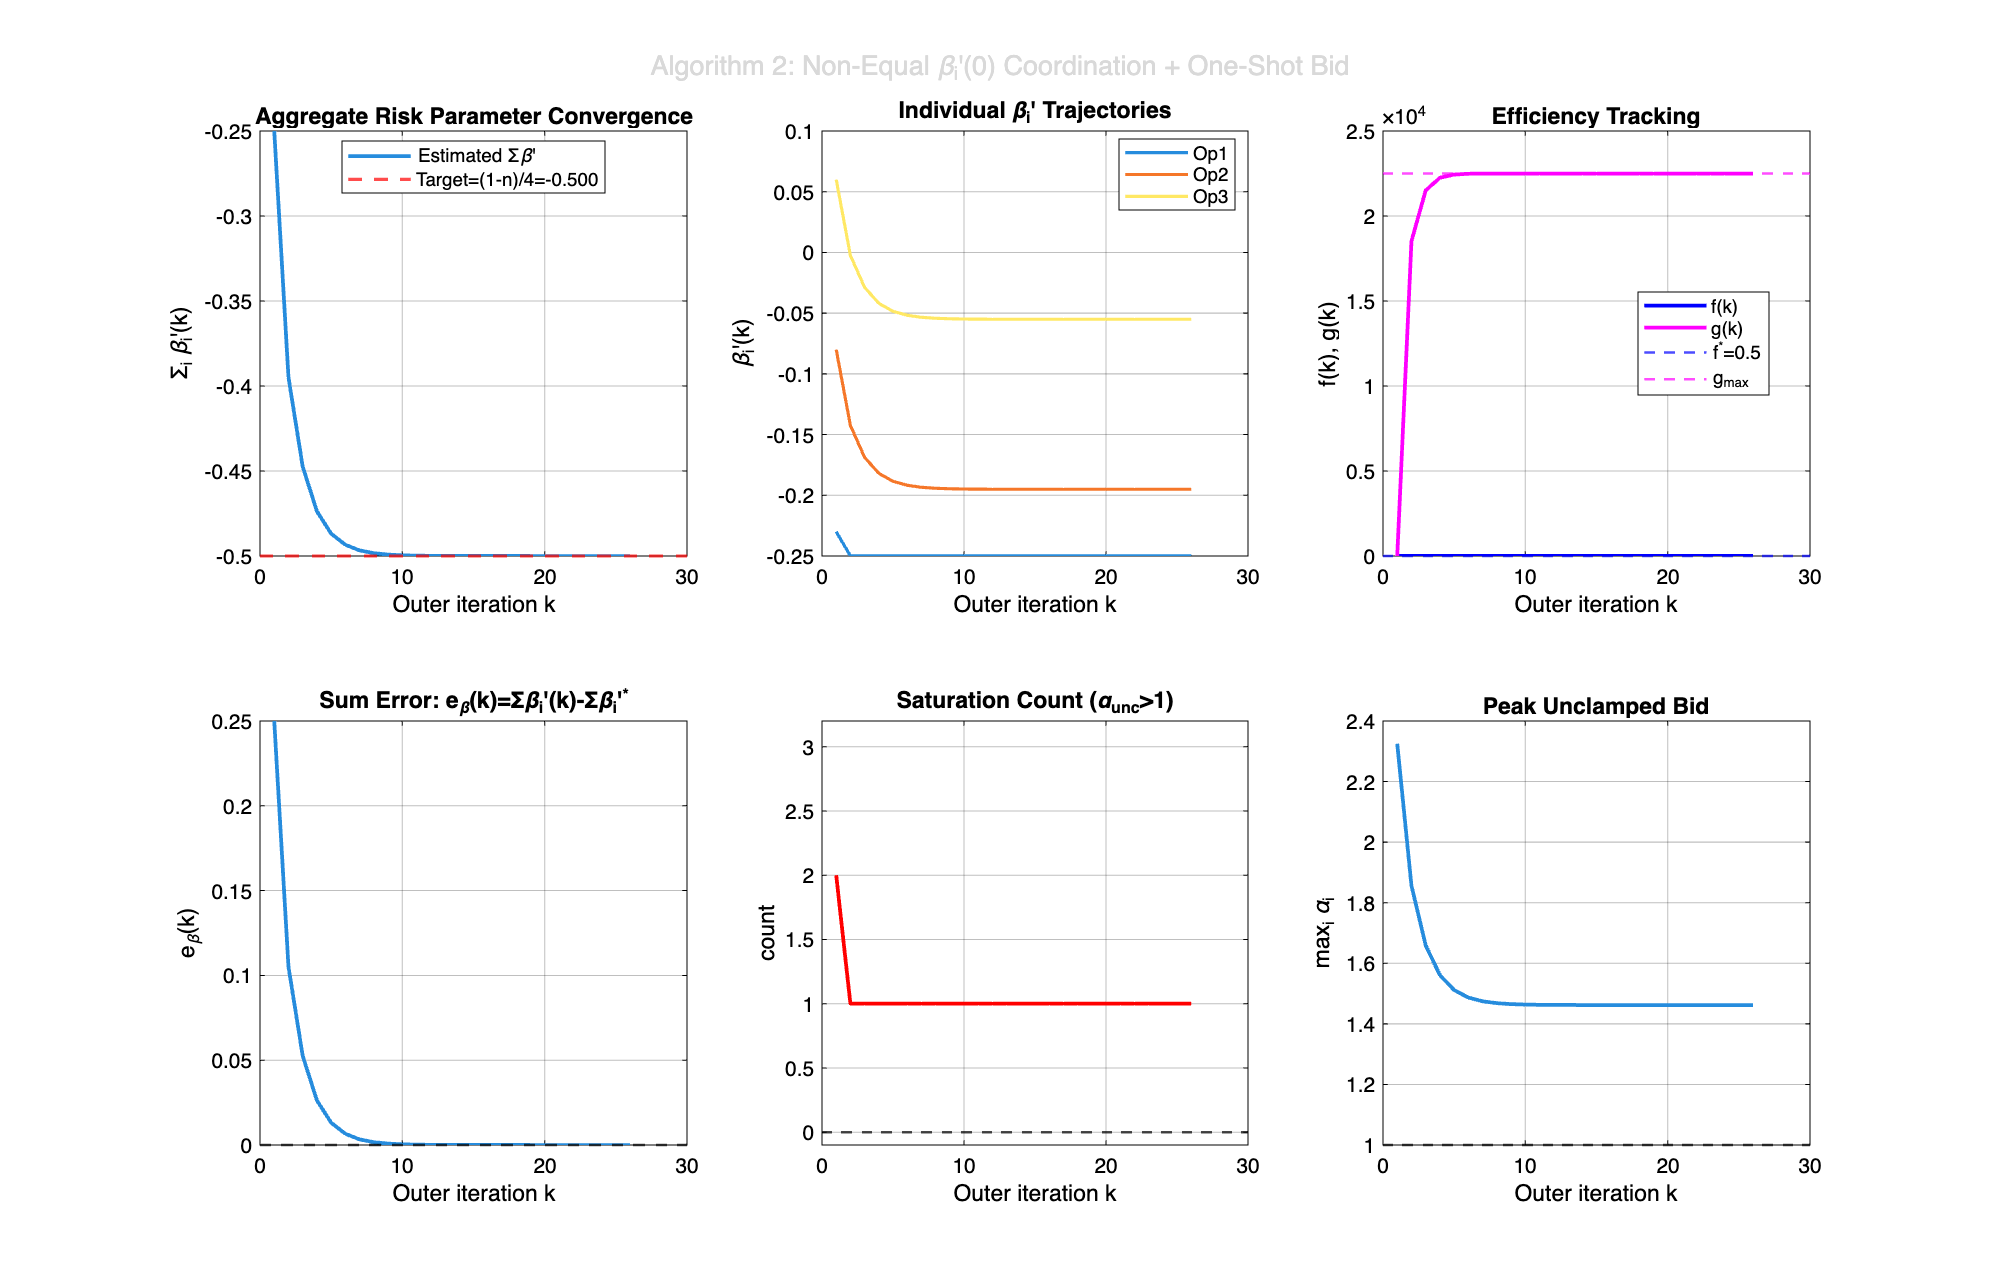
\includegraphics[width=1\linewidth]{figures/algorithm2_results.png}
    \caption{Algorithm~2 single-scenario diagnostics: convergence of $\sum\beta_i'$, individual $\beta_i'$, efficiency metrics, and saturation count.}
    \label{fig:algo2_single}
\end{figure}

\begin{figure}[hbt!]
    \centering
    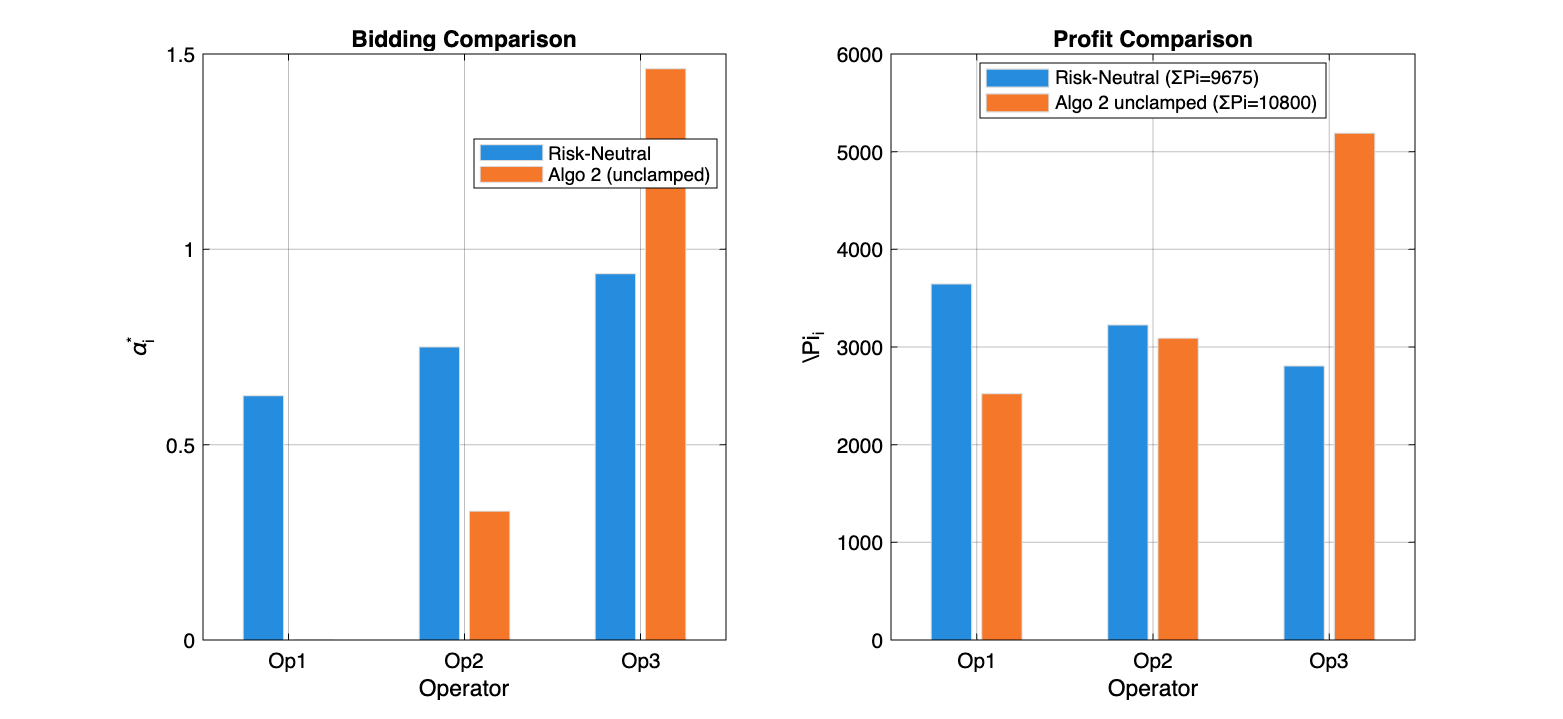
\includegraphics[width=1\linewidth]{figures/algorithm2_bidding_comparison.png}
    \caption{Algorithm~2 bidding/profit comparison under the unclamped $\alpha_i$ assumption.}
    \label{fig:algo2_bidprofit}
\end{figure}

\begin{figure}[hbt!]
    \centering
    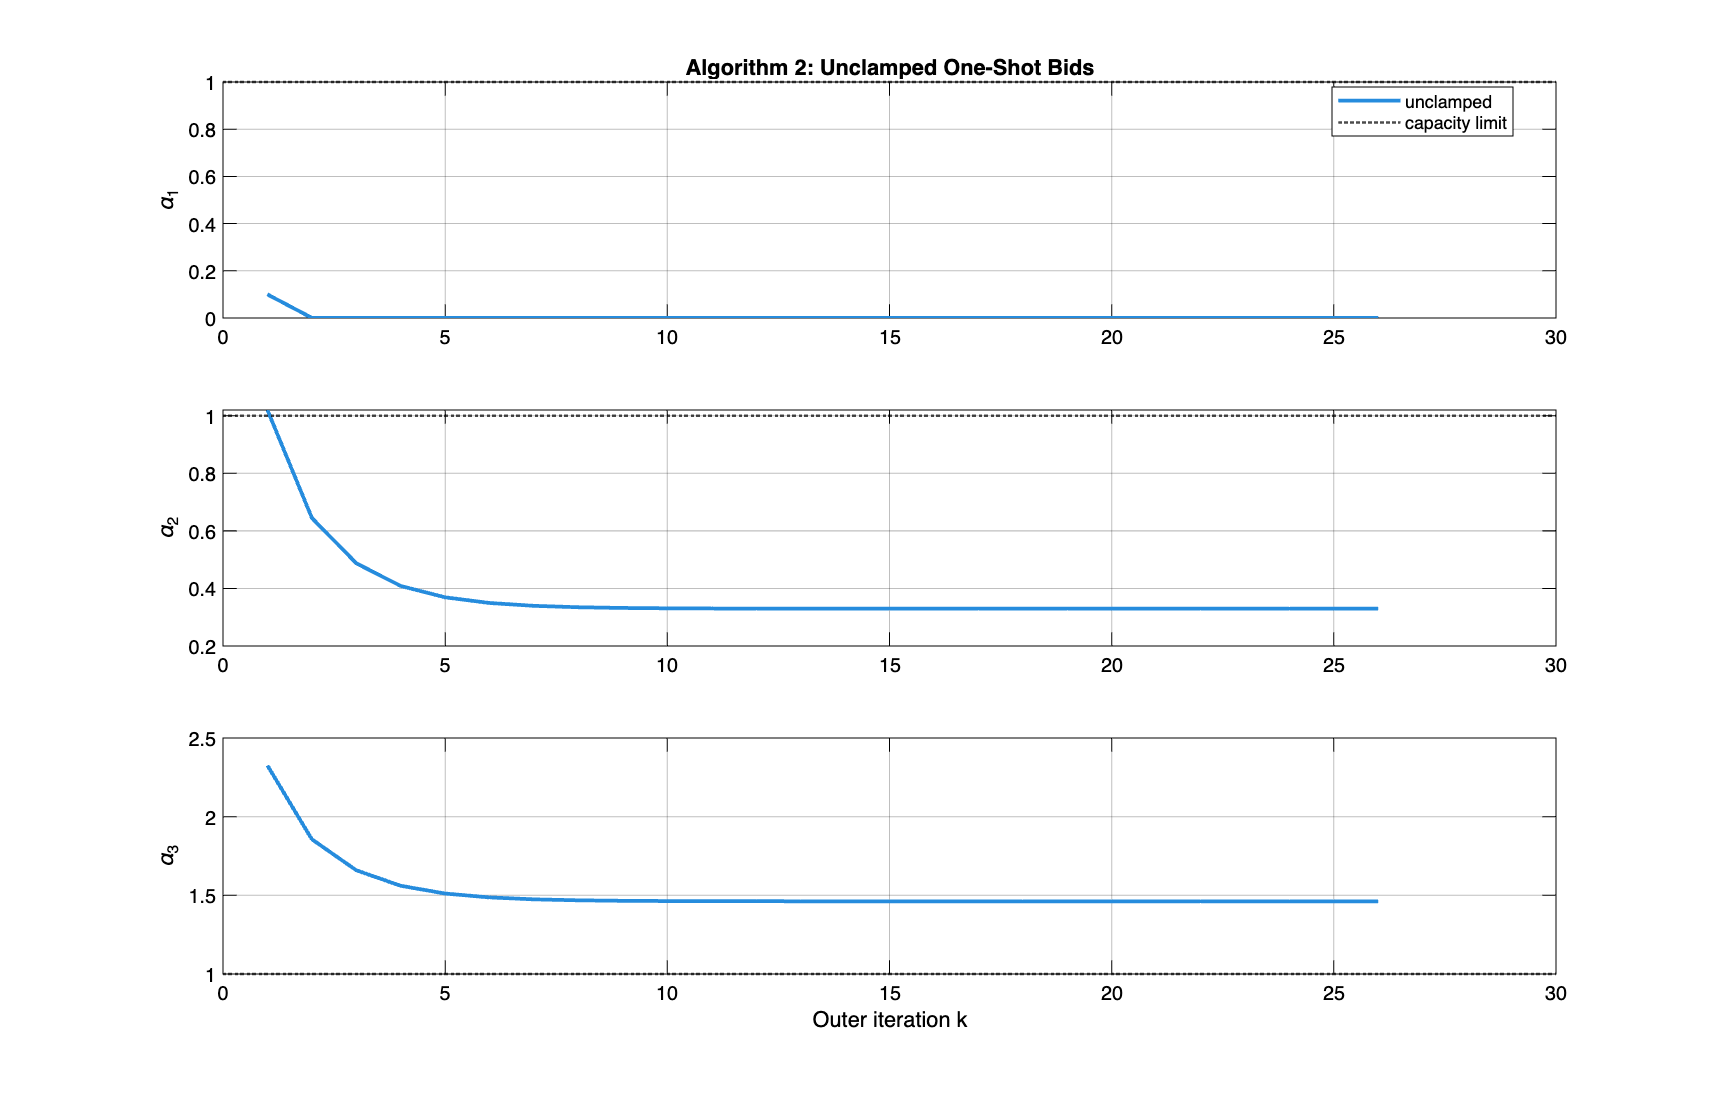
\includegraphics[width=1\linewidth]{figures/algorithm2_alpha_unclamped.png}
    \caption{Algorithm~2 one-shot bid trajectories under the unclamped $\alpha_i$ assumption, with capacity limit shown for reference.}
    \label{fig:algo2_clamp}
\end{figure}

\begin{table}[h]
\centering
\caption{Test cases with initial transformed risk parameters $\beta_i' = a_2\beta_i$}
\label{tab:test_cases}
\begin{tabular}{lcccc}
\hline
Test case & $\beta_1'$ & $\beta_2'$ & $\beta_3'$ & Risk Profile \\
\hline
I & 0 & 0 & 0 & Risk-neutral \\
II & -1 & -1 & -1 & Risk-seeking \\
III & 1 & 1 & 1 & Risk-averse \\
IV & -1 & 1 & 1 & Mixed \\
V & -0.25 & 0 & 0.20 & Mixed \\
VI & -0.25 & 0 & 0 & Mixed \\
\hline
\end{tabular}
\end{table}

\begin{figure}[hbt!]
    \centering
    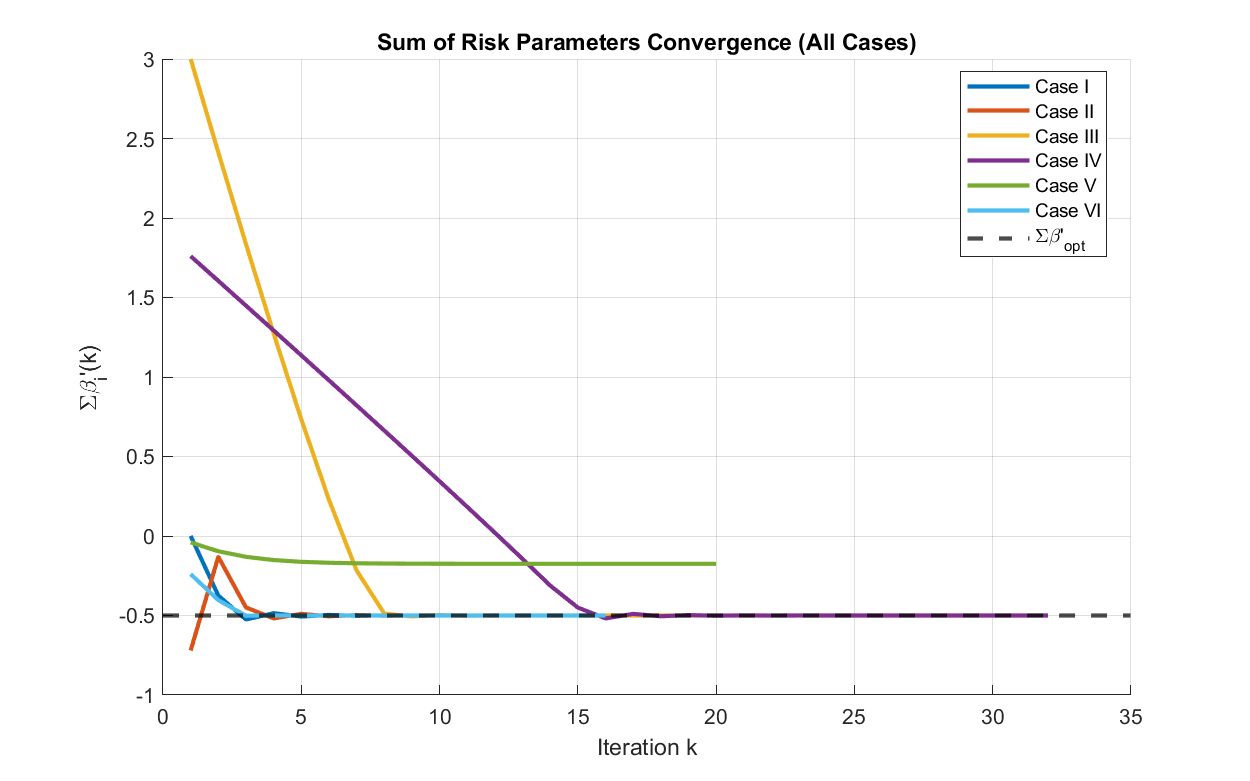
\includegraphics[width=1\linewidth]{figures/sum_beta_convergence_all_cases.png}
    \caption{Convergence of $\sum\beta_i'$ for all test cases. Each case converges to the Pareto-optimal sum $\sum\beta_i'^* = (1-n)/4 = -0.5$.}
    \label{fig:sum_beta_all}
\end{figure}

\begin{figure}[hbt!]
    \centering
    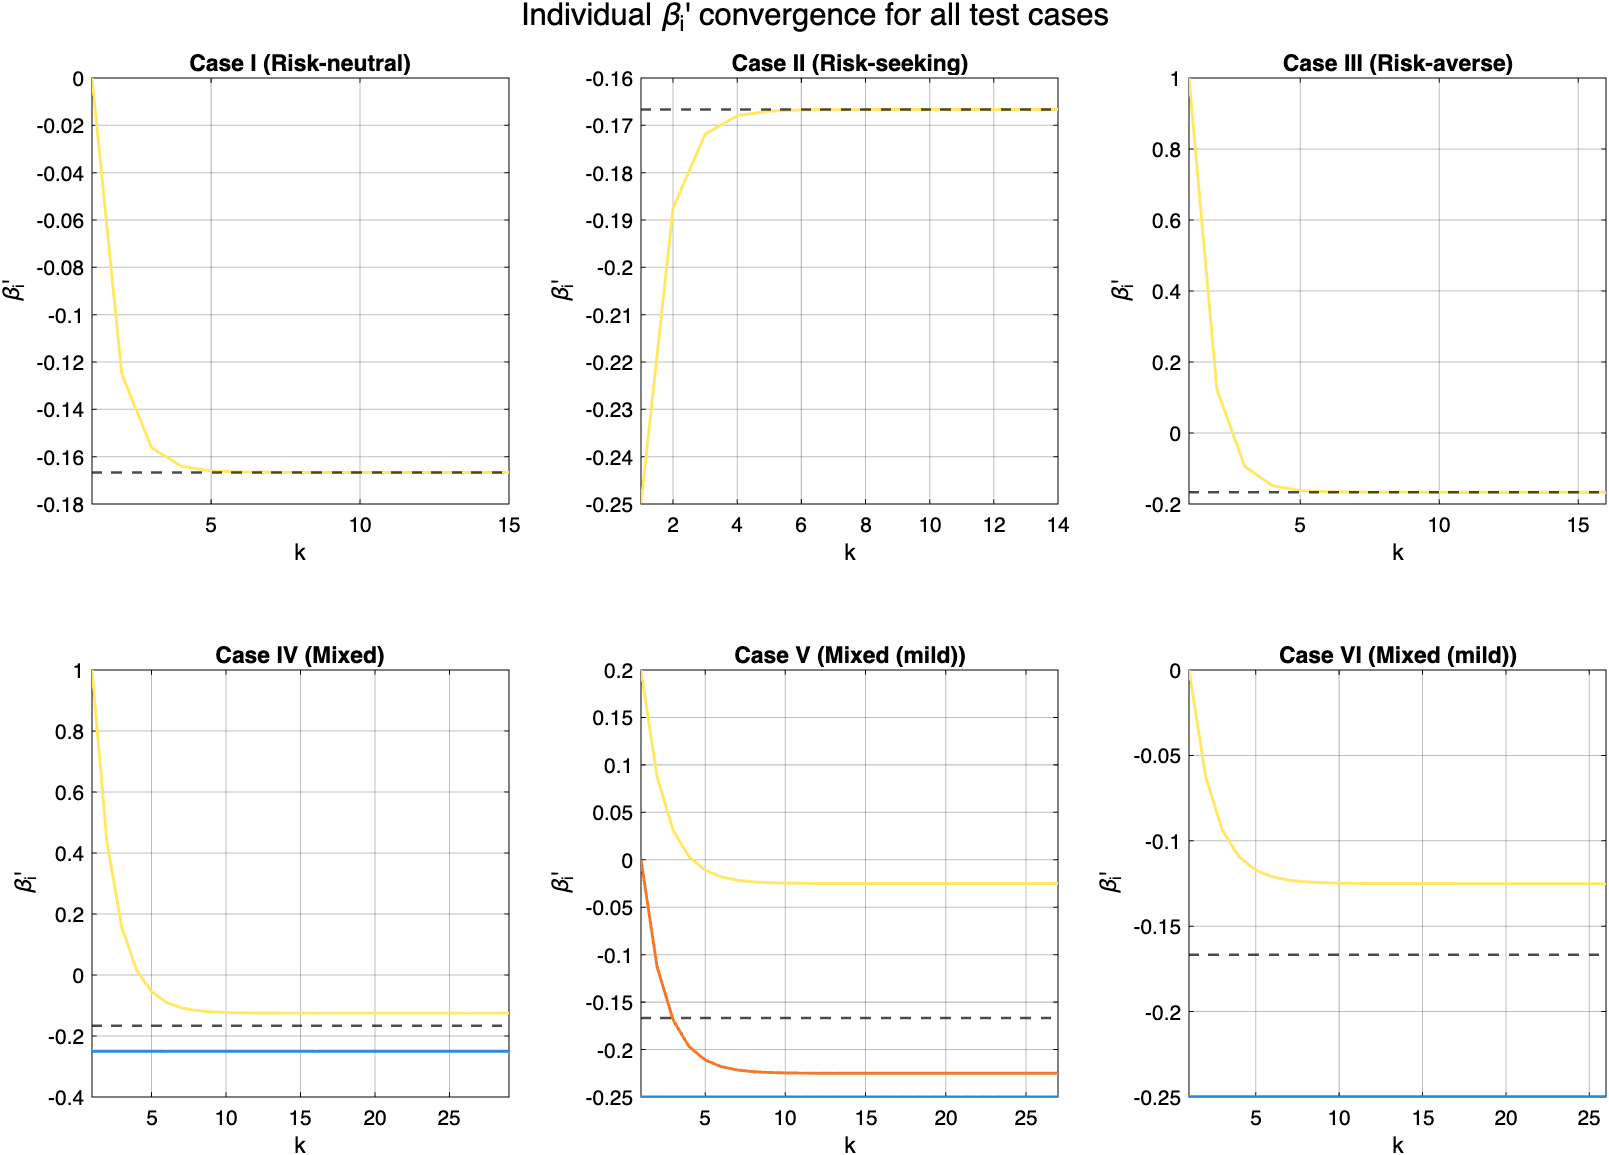
\includegraphics[width=1\linewidth]{figures/beta_individual_all_cases.png}
    \caption{Individual $\beta_i'$ convergence for each test case. Most cases achieve the Pareto-optimal sum; cases with capacity-constrained operators may converge to alternative equilibria (see Remark~1).}
    \label{fig:beta_individual}
\end{figure}

\begin{figure}[hbt!]
    \centering
    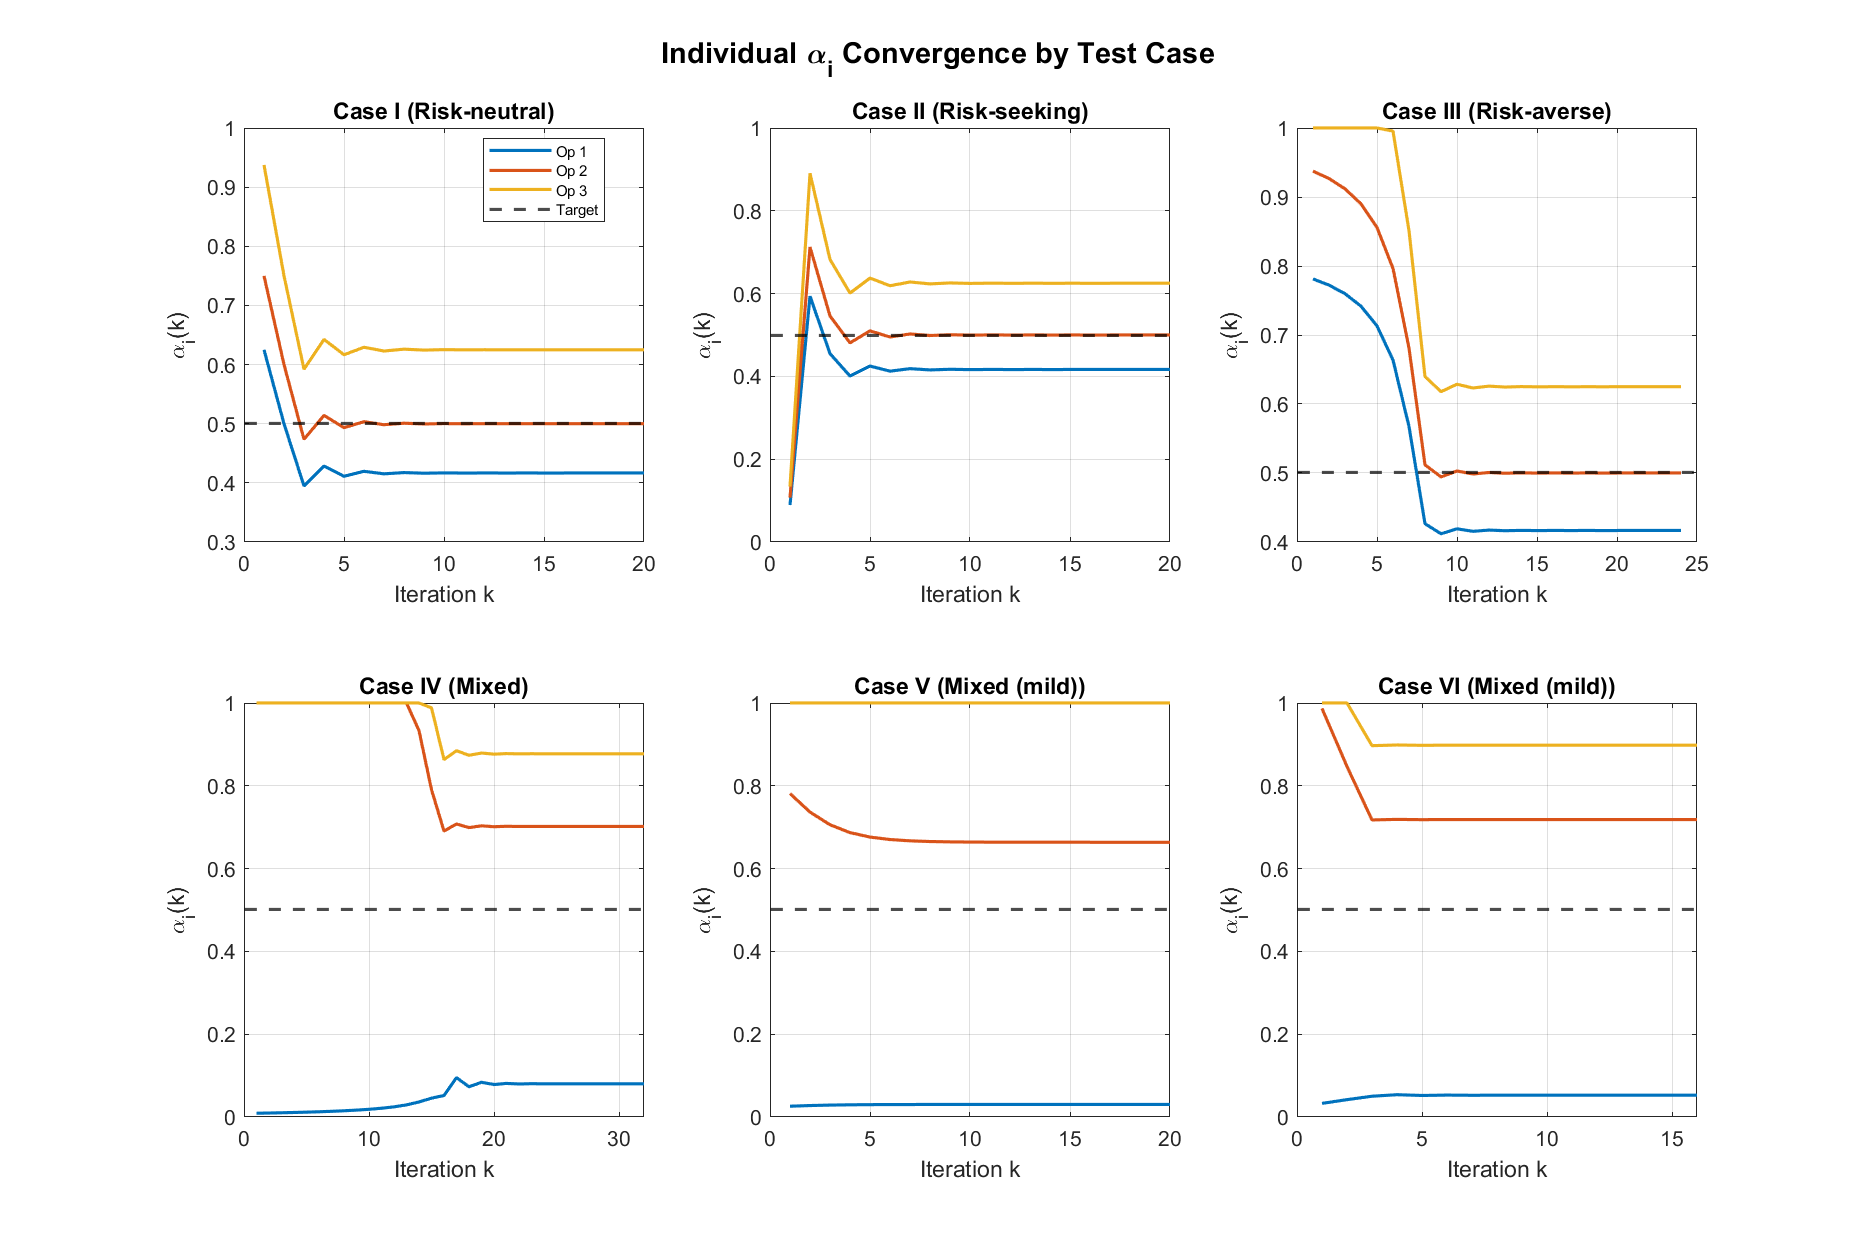
\includegraphics[width=1\linewidth]{figures/alpha_individual_all_cases.png}
    \caption{Individual $\alpha_i$ convergence for each test case. Bidding fractions adjust to achieve $f(\alpha) = 0.5$.}
    \label{fig:alpha_individual}
\end{figure}

Figure~\ref{fig:sum_beta_all} shows the convergence of the aggregate risk parameter $\sum\beta_i'$ for all test cases. Despite vastly different initial conditions ranging from risk-neutral (Case~I) to risk-seeking (Case~II) to risk-averse (Case~III) to mixed profiles (Cases~IV--VI), most cases converge to the Pareto-optimal value $\sum\beta_i'^* = (1-n)/4 = -0.5$ as predicted by Theorem~2. For cases with highly asymmetric initial risk preferences where capacity constraints bind (see Remark~1), the algorithm may converge to a different $\sum\beta_i'$ while still driving $f(\alpha)$ close to $0.5$ under the unclamped-bid model. Figure~\ref{fig:beta_individual} provides a detailed view of individual $\beta_i'$ trajectories within each case, showing how operators with different initial risk preferences adapt their parameters.

Figure~\ref{fig:alpha_individual} shows the corresponding evolution of bidding fractions $\alpha_i$. As the risk parameters converge, the bidding strategies adjust to achieve $f(\alpha) = 0.5$, confirming the Nash equilibrium behavior characterized in Lemma~2. Figures~\ref{fig:algo2_single}, \ref{fig:algo2_bidprofit}, and~\ref{fig:algo2_clamp} further illustrate the single-scenario dynamics of Algorithm~2 under the unclamped-bid assumption. The impact of the risk-parameter updates on market efficiency is illustrated in Figures~\ref{fig:f_all} and~\ref{fig:S_all}, where the aggregate bidding fraction $f(\alpha)$ converges to $1/2$ and the error signal $|S|$ decreases below the convergence tolerance for all test cases.

\begin{figure}[hbt!]
    \centering
    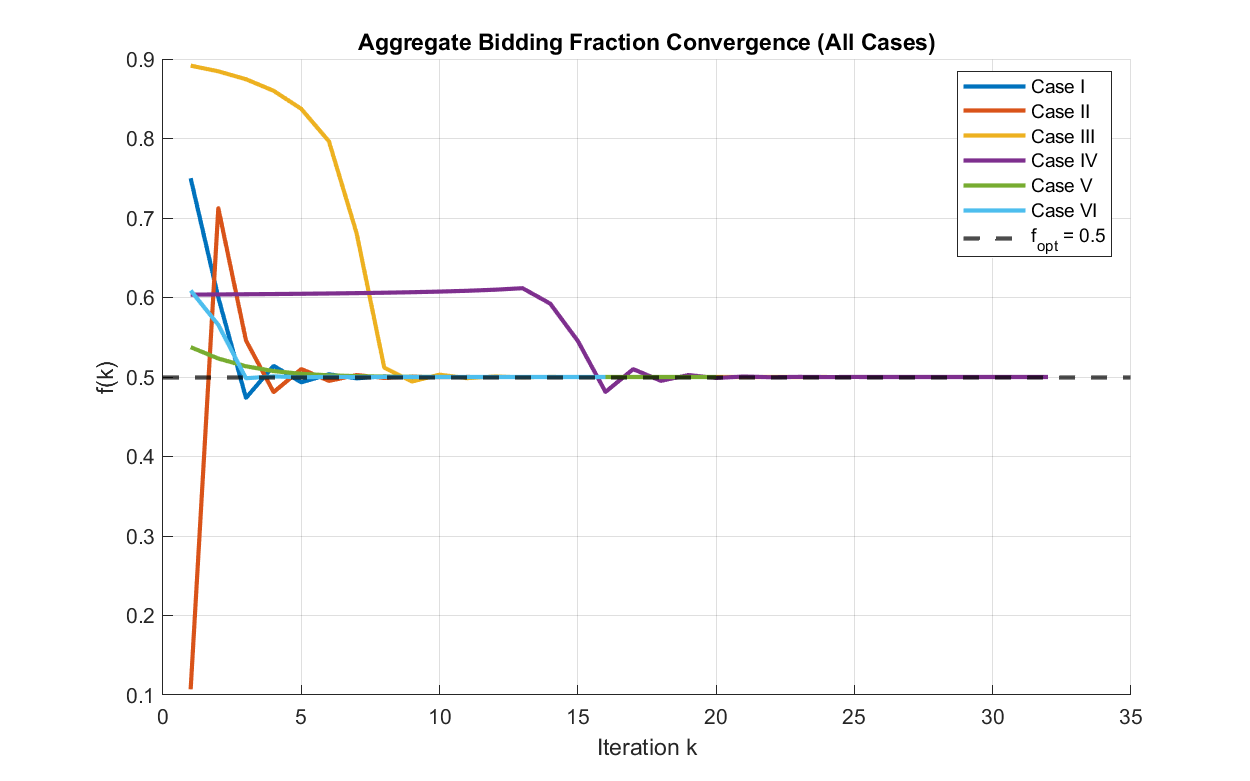
\includegraphics[width=1\linewidth]{figures/f_convergence_all_cases.png}
    \caption{Convergence of aggregate bidding fraction $f(\alpha)$ to Pareto target $0.5$ for all test cases.}
    \label{fig:f_all}
\end{figure}

\begin{figure}[hbt!]
    \centering
    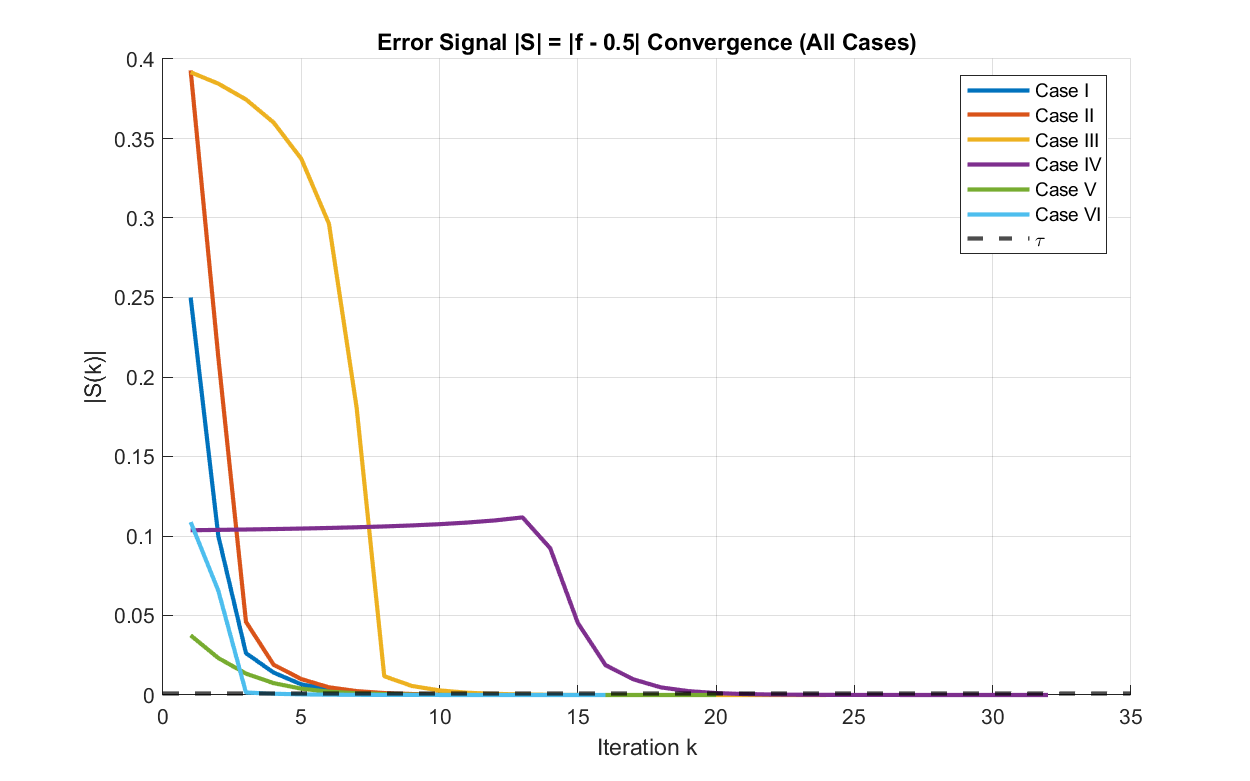
\includegraphics[width=1\linewidth]{figures/S_convergence_all_cases.png}
    \caption{Convergence of error signal $|S| = |f - 0.5|$ (log scale) for all test cases.}
    \label{fig:S_all}
\end{figure}

\begin{figure}[hbt!]
    \centering
    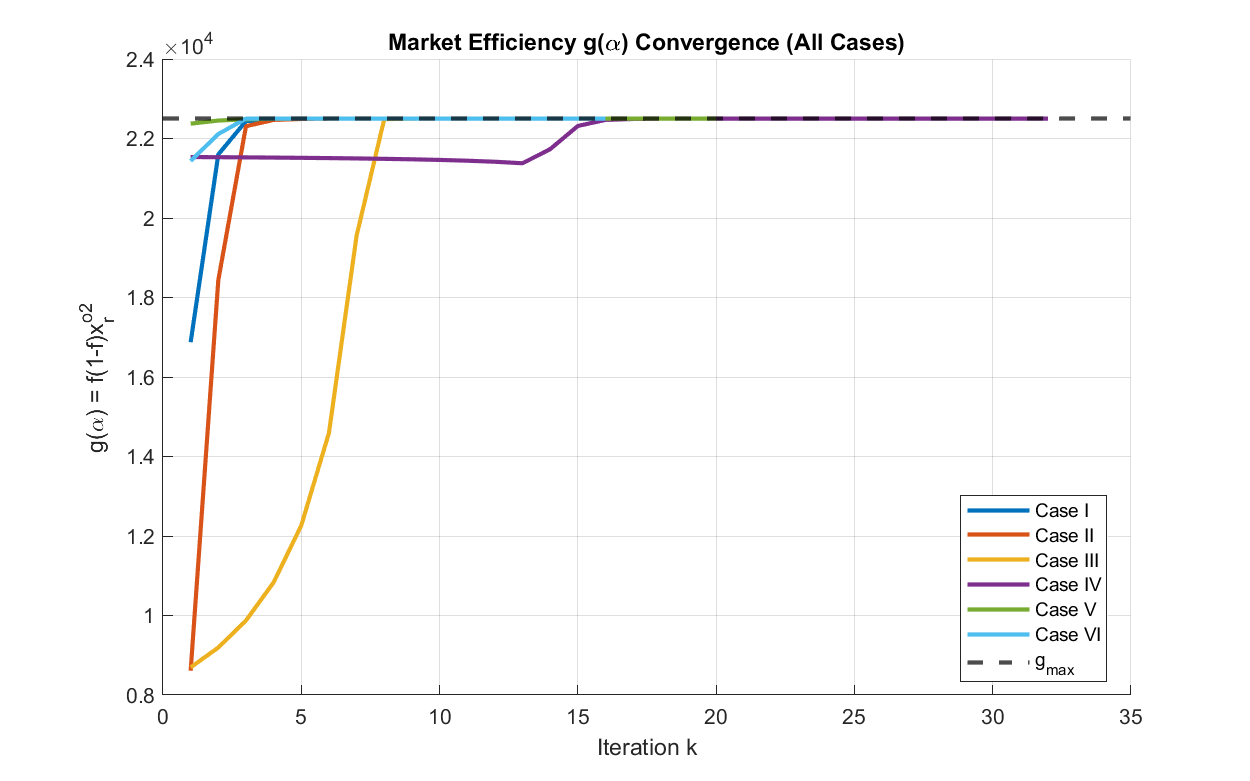
\includegraphics[width=1\linewidth]{figures/g_convergence_all_cases.png}
    \caption{Convergence of market efficiency $g(\alpha) = f(1-f)(x_r^o)^2$ to maximum value $g_{\max} = 0.25(x_r^o)^2$ for all test cases.}
    \label{fig:g_all}
\end{figure}

\begin{figure}[hbt!]
    \centering
    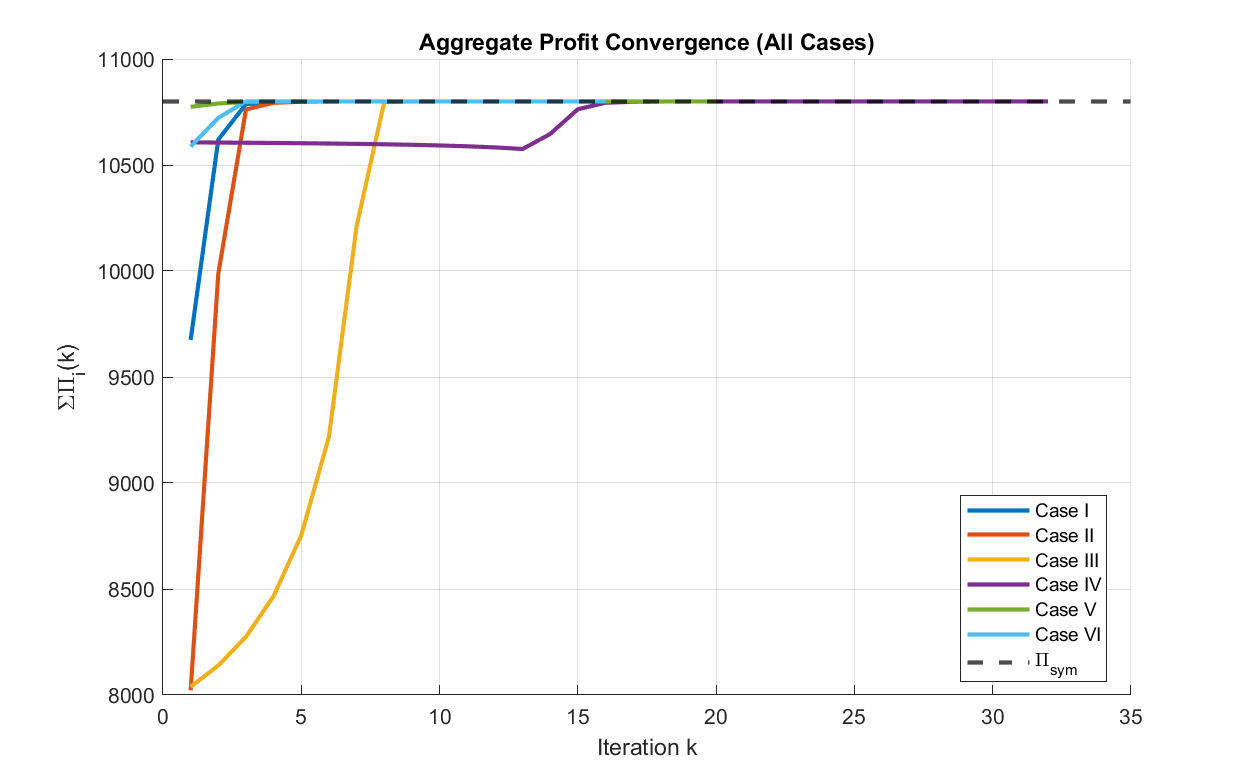
\includegraphics[width=1\linewidth]{figures/profit_convergence_all_cases.png}
    \caption{Convergence of aggregate profit $\sum\Pi_i$ for all test cases.}
    \label{fig:profit_all}
\end{figure}

Figure~\ref{fig:g_all} demonstrates that market efficiency $g(\alpha)$ converges to its maximum value $g_{\max} = 0.25(x_r^o)^2 = 22{,}500$ for all test cases, confirming that the distributed algorithm successfully achieves Pareto optimality. Figure~\ref{fig:profit_all} shows the corresponding convergence of aggregate profits $\sum\Pi_i$.

Notably, for mixed risk profiles where some operators are risk-seeking while others are risk-averse (e.g., Case~V), the unconstrained model can produce $\alpha_i>1$ for risk-averse operators, as discussed in Remark~1. In such cases, the aggregate risk parameter $\sum\beta_i'$ may not converge exactly to $(1-n)/4$; yet the algorithm still drives $f(\alpha)$ toward $0.5$ and near-Pareto aggregate profit. This demonstrates the robustness of the distributed approach under heterogeneous risk preferences.

These results validate that the proposed distributed algorithm achieves Pareto-enhanced Nash equilibria using only local computations and minimal information exchange. Regardless of initial risk preferences, the algorithm guides all operators toward the collective optimum. In particular, the renewable operators do not require knowledge of other agents' forecasts, cost parameters, or private objectives, yet collectively achieve the same performance as a centralized optimizer. This highlights the practicality of the proposed framework for real-time electricity markets with decentralized renewable participants.
\end{comment}

\section{Conclusion}

This paper presented a risk-aware bidding framework in which the risk sensitivity parameter $\beta_i$ acts as a coordination variable for renewable generation operators in electricity markets. We showed that the noncooperative game admits structured Nash equilibria and that, by appropriate risk allocation, these equilibria can recover Pareto-efficient aggregate outcomes. In particular, the analysis established explicit relationships between risk parameters, bidding coefficients, and market efficiency.

A distributed consensus-based implementation was developed for the one-shot strategy, allowing each operator to estimate required aggregate quantities using only local communication. The illustrative example confirmed that the distributed Algorithm~1 reproduces the targeted bidding behavior without centralized disclosure of private forecasts or cost data. When the no-overbidding constraint is active, a minor extension using a third consensus protocol allows each operator to determine its constrained bid locally after recovering the aggregate saturation quantities $\sum_{j\in\Omega_{\rm ERS}}\eta_j$ and $\sum_{j\not\in\Omega_{\rm ERS}}\eta_j$ through neighborhood communication alone.

A detailed overbidding analysis established per-operator saturation thresholds from~\eqref{eq:overbid_bound} and showed that operators with smaller capacity shares saturate first under a common risk parameter. The individual profit analysis revealed that the no-overbidding projection shifts $f(\boldsymbol{\alpha})$ below $\tfrac{1}{2}$ and reduces the payoff of all operators through the shared market-clearing term, not only those whose bids are clamped. This individual-level effect, quantified via~\eqref{eq:Pi_i} and illustrated numerically in the constrained Scenario~2 study, demonstrates that the performance impact of feasibility constraints is collective rather than local.

Overall, the results demonstrate that risk-aware design can align self-interested bidding with improved collective efficiency while preserving decentralization and privacy. Future work will incorporate network congestion and locational pricing, extend to non-Gaussian uncertainty structures and time-varying operator participation, and analyze robustness under communication delay, packet loss, and adversarial behavior.

\bibliographystyle{IEEEtran}
\bibliography{references}

\end{document}